\documentclass[10pt, xcolor=dvipsnames]{beamer}
% =====================================================================
% Preámbulo común — Diapositivas Magistrales, Econometría Avanzada
% =====================================================================
% Se incluye con % =====================================================================
% Preámbulo común — Diapositivas Magistrales, Econometría Avanzada
% =====================================================================
% Se incluye con % =====================================================================
% Preámbulo común — Diapositivas Magistrales, Econometría Avanzada
% =====================================================================
% Se incluye con \input{preambulo/preambulo-magistral} DESPUÉS de
% \documentclass[<tam>pt, xcolor=dvipsnames]{beamer} en cada archivo.
%
% Lo único que debe quedar en cada .tex individual es:
%   1) \documentclass[...]{beamer}      (el tamaño de fuente puede variar)
%   2) \input{preambulo/preambulo-magistral}
%   3) \subtitle{...}                   (título de la clase puntual)
% Todo lo demás (paquetes, macros, tema, título, autor, hypersetup, etc.)
% vive aquí para poder hacer cambios globales en un solo lugar.
% =====================================================================

% ---------------------------------------------------------------------
% 1. Codificación, idioma y fuentes
% ---------------------------------------------------------------------
\usepackage{etex}
\usepackage[utf8]{inputenc}
\usepackage[T1]{fontenc}
\usepackage[spanish,es-nodecimaldot]{babel}
\usepackage{lmodern}
\usepackage{type1cm}
\usepackage{textcomp}

% ---------------------------------------------------------------------
% 2. Matemáticas y símbolos
% ---------------------------------------------------------------------
\usepackage{amsmath,amssymb,amsthm,amsfonts}
\usepackage{bbm}
\usepackage{bm}

% ---------------------------------------------------------------------
% 3. Bibliografía y citas
% ---------------------------------------------------------------------
\usepackage[round]{natbib}
\bibliographystyle{erae}
\usepackage{bibentry}
\usepackage{url}
\let\htmlstyloaded=\relax

% Las citas se muestran en marrón para distinguirlas del contenido.
\let\oldcitet=\citet
\renewcommand{\citet}[1]{\textcolor{brown}{\oldcitet{#1}}}
\let\oldcitep=\citep
\renewcommand{\citep}[1]{\textcolor{brown}{\oldcitep{#1}}}
\let\oldcite=\cite
\renewcommand{\cite}[1]{\textcolor{brown}{\oldcite{#1}}}

% ---------------------------------------------------------------------
% 4. Figuras, tablas y colores
% ---------------------------------------------------------------------
\usepackage{float}
\usepackage{graphicx}
\usepackage{subcaption}
\usepackage[font={footnotesize}]{caption}
\usepackage{lscape}
\usepackage{longtable}
\usepackage{booktabs}
\usepackage{multirow}
\usepackage{array}
\usepackage[flushleft]{threeparttable}
\usepackage{color, colortbl}
\usepackage{eso-pic}
\usepackage{chngcntr}
\usepackage{adjustbox}
\usepackage{pdfpages}
\usepackage{media9}

% siunitx: usado para alinear/formatear números en tablas
\usepackage{siunitx}
\sisetup{
	detect-mode,
	tight-spacing		= true,
	group-digits		= false ,
	input-signs		= ,
	input-symbols		= ( ) [ ] - + *,
	input-open-uncertainty	= ,
	input-close-uncertainty	= ,
	table-align-text-post	= false
}

% ---------------------------------------------------------------------
% 5. TikZ / PGFPlots
% ---------------------------------------------------------------------
\usepackage{tikz}
\usepackage{pgfplots}
\usepgfplotslibrary{dateplot}
\usetikzlibrary{arrows,calc, patterns, positioning, shapes.geometric, decorations.pathreplacing,decorations.markings}

% ---------------------------------------------------------------------
% 6. Misceláneos de formato
% ---------------------------------------------------------------------
\usepackage{setspace}
\usepackage{lipsum}
\usepackage{framed}
\usepackage{mdframed}
\usepackage{fancyhdr}
\usepackage{beamerfoils}
\usepackage{pifont}
\usepackage{ragged2e}
\usepackage{xspace}
\usepackage{appendixnumberbeamer}
\usepackage[scale=2]{ccicons}
\usepackage[most]{tcolorbox}
\usepackage{enumitem}
\setbeamertemplate{note page}[plain]

% ---------------------------------------------------------------------
% 7. Hyperref (debe cargarse después de la mayoría de paquetes)
% ---------------------------------------------------------------------
\usepackage{hyperref}
\hypersetup {
	pdftitle={General},
	pdfauthor={Manuel Fern\'{a}ndez},
	colorlinks=true,
	citecolor=brown,
	linkcolor=black,
	urlcolor=blue
}
\makeatletter
\renewcommand{\hyper@natlinkstart}[1]{}
\renewcommand{\hyper@natlinkend}{}
\renewcommand{\hyper@natlinkbreak}[2]{#1}
\makeatother

% =====================================================================
% 8. Tema Beamer (metropolis)
% =====================================================================
\usetheme{metropolis}
\newcommand{\themename}{\textbf{\textsc{metropolis}}\xspace}
\metroset{sectionpage=none}

\setbeamerfont{citep}{family=\rm}
\setbeamerfont{caption}{size=\scriptsize}
\setbeamerfont{normal text}{size=7pt}

%\setcounter{tocdepth}{1}
\setbeamertemplate{section in toc}[sections numbered]
\AtBeginSection[]{
  \begin{frame}
  \vfill
  \centering
  \begin{beamercolorbox}[sep=8pt,center,shadow=true,rounded=true]{title}
    \usebeamerfont{title}\insertsectionhead\par%
  \end{beamercolorbox}
  \vfill
  \end{frame}
}
% NOTA: \setbeamercolor{button}, \setbeamercovered{invisible} y
% \AtBeginSubsection NO están aquí porque sólo algunas clases los usaban
% en el original (afectan botones de hipervínculo, el efecto de \pause,
% y los separadores de \subsection). Se preservan como "ajustes locales"
% en los .tex que ya los tenían, justo después de \input{preambulo}.

% =====================================================================
% 9. Macros de Estout (tablas de resultados)
% =====================================================================
\newcommand{\sym}[1]{\rlap{#1}}% Thanks to David Carlisle
\let\estinput=\input% define a new input command so that we can still flatten the document
\newcommand{\estwide}[3]{
	\vspace{.75ex}{
		\begin{tabular*}
			{\textwidth}{@{\hskip\tabcolsep\extracolsep\fill}l*{#2}{#3}}
			\toprule
			\estinput{#1}
			\bottomrule
			\addlinespace[.75ex]
		\end{tabular*}
	}
}
\newcommand{\estauto}[3]{
	\vspace{.75ex}{
		\begin{tabular}{l*{#2}{#3}}
			\toprule
			\estinput{#1}
			\bottomrule
			\addlinespace[.75ex]
		\end{tabular}
	}
}
% Allow line breaks with \\ in specialcells
\newcommand{\specialcell}[2][c]{%
	\begin{tabular}[#1]{@{}c@{}}#2\end{tabular}}

% =====================================================================
% 10. Notas y fuentes al pie de figuras/tablas
% =====================================================================
% Note/Source/Text after Tables
\newcommand{\figtext}[1]{
	\vspace{-1.9ex}
	\captionsetup{justification=justified,font=footnotesize}
	\caption*{\hspace{6pt}\hangindent=1.5em #1}
}
\newcommand{\fignote}[1]{\figtext{\emph{Note:~}~#1}}
\newcommand{\figsource}[1]{\figtext{\emph{Source:~}~#1}}
% Add significance note with \starnote
\newcommand{\starnote}{\figtext{* p $<$ 0.10 ** p $<$ 0.05 *** p $<$ 0.01. }}

% =====================================================================
% 11. Entornos tipo teorema (en español)
% =====================================================================
\newtheorem{Prop}{Proposition}[section]
\newtheorem{Def}{Definition}
%\newtheorem{Assum}{Assumption}
%\newtheorem{Question}{Question}
%\newtheorem{Comment}{Comment}
%\theoremstyle{plain}
%\numberwithin{Assum}{section}
%\numberwithin{figure}{section}
%\numberwithin{equation}{section}
%\numberwithin{Def}{section}

\newenvironment{Teorema}[1][Teorema.]{\begin{trivlist}
		\item[\hskip \labelsep {\bfseries #1}]}{\end{trivlist}}
\newenvironment{Corolario}[1][Corolario.]{\begin{trivlist}
		\item[\hskip \labelsep {\bfseries #1}]}{\end{trivlist}}
\newenvironment{Definicion}[1][Definición.]{\begin{trivlist}
		\item[\hskip \labelsep {\bfseries #1}]}{\end{trivlist}}
\newenvironment{Lema}[1][Lema.]{\begin{trivlist}
		\item[\hskip \labelsep {\bfseries #1}]}{\end{trivlist}}
\newenvironment{Ejemplo}[1][Ejemplo.]{\begin{trivlist}
		\item[\hskip \labelsep {\bfseries #1}]}{\end{trivlist}}

\newenvironment{myindentpar}[1]%
{\begin{list}{}%
		{\setlength{\leftmargin}{#1}}%
		\item[]%
	}
	{\end{list}}

% =====================================================================
% 12. Notación matemática y econométrica
% =====================================================================
\newcommand{\plim}{\operatornamewithlimits{plim}}
\newcommand{\Var}{\operatorname{Var}}
\newcommand{\pderiv}[2]{\frac{\partial #1}{\partial #2}}
\newcommand{\spderiv}[2]{\frac{\partial^2 #1}{\partial #2^2}}
\newcommand{\xderiv}[3]{\frac{\partial^2 #1}{\partial #2 \partial #3}}
\newcommand{\argmin}{\operatornamewithlimits{arg\,min}}
\newcommand{\argmax}{\operatornamewithlimits{arg\,max}}
\newcommand{\amax}{\operatornamewithlimits{max}}
\newcommand{\amin}{\operatornamewithlimits{min}}
\newcommand*\circled[1]{\tikz[baseline=(char.base)]{\node[shape=circle,draw,inner sep=1pt] (char) {#1};}}
\newcommand{\indep}{\perp \!\!\! \perp}
\makeatletter
\newcommand{\distas}[1]{\mathbin{\overset{#1}{\kern\z@\sim}}}%
\newsavebox{\mybox}\newsavebox{\mysim}
\newcommand{\distras}[1]{%
	\savebox{\mybox}{\hbox{\kern3pt$\scriptstyle#1$\kern3pt}}%
	\savebox{\mysim}{\hbox{$\sim$}}%
	\mathbin{\overset{#1}{\kern\z@\resizebox{\wd\mybox}{\ht\mysim}{$\sim$}}}%
}
\makeatother

\DeclareMathOperator{\EX}{\mathbb{E}}% expected value
\newcommand{\Prob}[1]{\text{Pr}\left[#1\right]}
\newcommand{\RK}[1]{\mathbb{R}^{#1}}
\newcommand{\HT}[1]{\mathbb{H}_{#1}}

% Vectores y matrices en negrilla (romana)
\newcommand{\xB}{\textbf{x}}
\newcommand{\yB}{\textbf{y}}
\newcommand{\zB}{\textbf{z}}
\newcommand{\wB}{\textbf{w}}
\newcommand{\eB}{\textbf{e}}
\newcommand{\vB}{\textbf{v}}
\newcommand{\AB}{\textbf{A}}
\newcommand{\XB}{\textbf{X}}
\newcommand{\YB}{\textbf{Y}}
\newcommand{\ZB}{\textbf{Z}}
\newcommand{\QB}{\textbf{Q}}
\newcommand{\WB}{\textbf{W}}

% Vectores griegos en negrilla
\newcommand{\betaB}{\boldsymbol{\beta}}
\newcommand{\gammaB}{\boldsymbol{\gamma}}
\newcommand{\alphaB}{\boldsymbol{\alpha}}
\newcommand{\thetaB}{\boldsymbol{\theta}}
\newcommand{\deltaB}{\boldsymbol{\delta}}
\newcommand{\phiB}{\boldsymbol{\phi}}
\newcommand{\epsilonB}{\boldsymbol{\epsilon}}
\newcommand{\etaB}{\boldsymbol{\eta}}
\newcommand{\betaBH}{\boldsymbol{\hat{\beta}}}
\newcommand{\betaH}{\hat{\beta}}

% Colores de énfasis
\newcommand{\brown}[1]{\textcolor{brown}{#1}}
\newcommand{\blue}[1]{\textcolor{blue}{#1}}
\newcommand{\red}[1]{\textcolor{red}{#1}}

% Espaciados usados en itemize/enumerate
\newcommand{\smallspace}{\vspace{0.1cm}}
\newcommand{\mediumspace}{\vspace{0.3cm}}
\newcommand{\largespace}{\vspace{6cm}}

% Tamaños de fuente auxiliares
\newcommand\fontvia{\fontsize{4}{6}\selectfont}
\newcommand\fontvib{\fontsize{5}{8}\selectfont}
\newcommand\fontvic{\fontsize{7}{10}\selectfont}
\newcommand\fontvid{\fontsize{8}{11}\selectfont}
\newcommand\fontvie{\fontsize{10}{11}\selectfont}

% Celdas de mapa de calor estilizado para la intuición de shift-share
% Monotone (brown) cell: value 0..100 -> brown intensity
\newcommand{\sharecell}[3]{%
  \pgfmathtruncatemacro{\vv}{#3}%
  \fill[brown!\vv!white] (#1,#2) rectangle ({#1+1},{#2+1});%
  \draw[gray!40] (#1,#2) rectangle ({#1+1},{#2+1});%
}
% Diverging (blue/red) cell: value -50..50 -> blue (neg) or red (pos)
\newcommand{\divcell}[3]{%
  \pgfmathtruncatemacro{\absvv}{abs(#3)*2}%
  \pgfmathtruncatemacro{\negflag}{(#3)<0 ? 1 : 0}%
  \ifnum\negflag=1
    \fill[blue!\absvv!white] (#1,#2) rectangle ({#1+1},{#2+1});%
  \else
    \fill[red!\absvv!white] (#1,#2) rectangle ({#1+1},{#2+1});%
  \fi
  \draw[gray!40] (#1,#2) rectangle ({#1+1},{#2+1});%
}
% Uniform cell: same color regardless of (col,row)
\newcommand{\unifcell}[3]{%
  \pgfmathtruncatemacro{\vv}{#3}%
  \fill[red!\vv!white] (#1,#2) rectangle ({#1+1},{#2+1});%
  \draw[gray!40] (#1,#2) rectangle ({#1+1},{#2+1});%
}

% =====================================================================
% 13. Datos de portada (comunes a todas las clases)
% =====================================================================
\title{Econometría Avanzada}
\author{Manuel Fernández}
\date{\today}
%\titlegraphic{\hfill\includegraphics[height=1.5cm]{logo.pdf}}
 DESPUÉS de
% \documentclass[<tam>pt, xcolor=dvipsnames]{beamer} en cada archivo.
%
% Lo único que debe quedar en cada .tex individual es:
%   1) \documentclass[...]{beamer}      (el tamaño de fuente puede variar)
%   2) % =====================================================================
% Preámbulo común — Diapositivas Magistrales, Econometría Avanzada
% =====================================================================
% Se incluye con \input{preambulo/preambulo-magistral} DESPUÉS de
% \documentclass[<tam>pt, xcolor=dvipsnames]{beamer} en cada archivo.
%
% Lo único que debe quedar en cada .tex individual es:
%   1) \documentclass[...]{beamer}      (el tamaño de fuente puede variar)
%   2) \input{preambulo/preambulo-magistral}
%   3) \subtitle{...}                   (título de la clase puntual)
% Todo lo demás (paquetes, macros, tema, título, autor, hypersetup, etc.)
% vive aquí para poder hacer cambios globales en un solo lugar.
% =====================================================================

% ---------------------------------------------------------------------
% 1. Codificación, idioma y fuentes
% ---------------------------------------------------------------------
\usepackage{etex}
\usepackage[utf8]{inputenc}
\usepackage[T1]{fontenc}
\usepackage[spanish,es-nodecimaldot]{babel}
\usepackage{lmodern}
\usepackage{type1cm}
\usepackage{textcomp}

% ---------------------------------------------------------------------
% 2. Matemáticas y símbolos
% ---------------------------------------------------------------------
\usepackage{amsmath,amssymb,amsthm,amsfonts}
\usepackage{bbm}
\usepackage{bm}

% ---------------------------------------------------------------------
% 3. Bibliografía y citas
% ---------------------------------------------------------------------
\usepackage[round]{natbib}
\bibliographystyle{erae}
\usepackage{bibentry}
\usepackage{url}
\let\htmlstyloaded=\relax

% Las citas se muestran en marrón para distinguirlas del contenido.
\let\oldcitet=\citet
\renewcommand{\citet}[1]{\textcolor{brown}{\oldcitet{#1}}}
\let\oldcitep=\citep
\renewcommand{\citep}[1]{\textcolor{brown}{\oldcitep{#1}}}
\let\oldcite=\cite
\renewcommand{\cite}[1]{\textcolor{brown}{\oldcite{#1}}}

% ---------------------------------------------------------------------
% 4. Figuras, tablas y colores
% ---------------------------------------------------------------------
\usepackage{float}
\usepackage{graphicx}
\usepackage{subcaption}
\usepackage[font={footnotesize}]{caption}
\usepackage{lscape}
\usepackage{longtable}
\usepackage{booktabs}
\usepackage{multirow}
\usepackage{array}
\usepackage[flushleft]{threeparttable}
\usepackage{color, colortbl}
\usepackage{eso-pic}
\usepackage{chngcntr}
\usepackage{adjustbox}
\usepackage{pdfpages}
\usepackage{media9}

% siunitx: usado para alinear/formatear números en tablas
\usepackage{siunitx}
\sisetup{
	detect-mode,
	tight-spacing		= true,
	group-digits		= false ,
	input-signs		= ,
	input-symbols		= ( ) [ ] - + *,
	input-open-uncertainty	= ,
	input-close-uncertainty	= ,
	table-align-text-post	= false
}

% ---------------------------------------------------------------------
% 5. TikZ / PGFPlots
% ---------------------------------------------------------------------
\usepackage{tikz}
\usepackage{pgfplots}
\usepgfplotslibrary{dateplot}
\usetikzlibrary{arrows,calc, patterns, positioning, shapes.geometric, decorations.pathreplacing,decorations.markings}

% ---------------------------------------------------------------------
% 6. Misceláneos de formato
% ---------------------------------------------------------------------
\usepackage{setspace}
\usepackage{lipsum}
\usepackage{framed}
\usepackage{mdframed}
\usepackage{fancyhdr}
\usepackage{beamerfoils}
\usepackage{pifont}
\usepackage{ragged2e}
\usepackage{xspace}
\usepackage{appendixnumberbeamer}
\usepackage[scale=2]{ccicons}
\usepackage[most]{tcolorbox}
\usepackage{enumitem}
\setbeamertemplate{note page}[plain]

% ---------------------------------------------------------------------
% 7. Hyperref (debe cargarse después de la mayoría de paquetes)
% ---------------------------------------------------------------------
\usepackage{hyperref}
\hypersetup {
	pdftitle={General},
	pdfauthor={Manuel Fern\'{a}ndez},
	colorlinks=true,
	citecolor=brown,
	linkcolor=black,
	urlcolor=blue
}
\makeatletter
\renewcommand{\hyper@natlinkstart}[1]{}
\renewcommand{\hyper@natlinkend}{}
\renewcommand{\hyper@natlinkbreak}[2]{#1}
\makeatother

% =====================================================================
% 8. Tema Beamer (metropolis)
% =====================================================================
\usetheme{metropolis}
\newcommand{\themename}{\textbf{\textsc{metropolis}}\xspace}
\metroset{sectionpage=none}

\setbeamerfont{citep}{family=\rm}
\setbeamerfont{caption}{size=\scriptsize}
\setbeamerfont{normal text}{size=7pt}

%\setcounter{tocdepth}{1}
\setbeamertemplate{section in toc}[sections numbered]
\AtBeginSection[]{
  \begin{frame}
  \vfill
  \centering
  \begin{beamercolorbox}[sep=8pt,center,shadow=true,rounded=true]{title}
    \usebeamerfont{title}\insertsectionhead\par%
  \end{beamercolorbox}
  \vfill
  \end{frame}
}
% NOTA: \setbeamercolor{button}, \setbeamercovered{invisible} y
% \AtBeginSubsection NO están aquí porque sólo algunas clases los usaban
% en el original (afectan botones de hipervínculo, el efecto de \pause,
% y los separadores de \subsection). Se preservan como "ajustes locales"
% en los .tex que ya los tenían, justo después de \input{preambulo}.

% =====================================================================
% 9. Macros de Estout (tablas de resultados)
% =====================================================================
\newcommand{\sym}[1]{\rlap{#1}}% Thanks to David Carlisle
\let\estinput=\input% define a new input command so that we can still flatten the document
\newcommand{\estwide}[3]{
	\vspace{.75ex}{
		\begin{tabular*}
			{\textwidth}{@{\hskip\tabcolsep\extracolsep\fill}l*{#2}{#3}}
			\toprule
			\estinput{#1}
			\bottomrule
			\addlinespace[.75ex]
		\end{tabular*}
	}
}
\newcommand{\estauto}[3]{
	\vspace{.75ex}{
		\begin{tabular}{l*{#2}{#3}}
			\toprule
			\estinput{#1}
			\bottomrule
			\addlinespace[.75ex]
		\end{tabular}
	}
}
% Allow line breaks with \\ in specialcells
\newcommand{\specialcell}[2][c]{%
	\begin{tabular}[#1]{@{}c@{}}#2\end{tabular}}

% =====================================================================
% 10. Notas y fuentes al pie de figuras/tablas
% =====================================================================
% Note/Source/Text after Tables
\newcommand{\figtext}[1]{
	\vspace{-1.9ex}
	\captionsetup{justification=justified,font=footnotesize}
	\caption*{\hspace{6pt}\hangindent=1.5em #1}
}
\newcommand{\fignote}[1]{\figtext{\emph{Note:~}~#1}}
\newcommand{\figsource}[1]{\figtext{\emph{Source:~}~#1}}
% Add significance note with \starnote
\newcommand{\starnote}{\figtext{* p $<$ 0.10 ** p $<$ 0.05 *** p $<$ 0.01. }}

% =====================================================================
% 11. Entornos tipo teorema (en español)
% =====================================================================
\newtheorem{Prop}{Proposition}[section]
\newtheorem{Def}{Definition}
%\newtheorem{Assum}{Assumption}
%\newtheorem{Question}{Question}
%\newtheorem{Comment}{Comment}
%\theoremstyle{plain}
%\numberwithin{Assum}{section}
%\numberwithin{figure}{section}
%\numberwithin{equation}{section}
%\numberwithin{Def}{section}

\newenvironment{Teorema}[1][Teorema.]{\begin{trivlist}
		\item[\hskip \labelsep {\bfseries #1}]}{\end{trivlist}}
\newenvironment{Corolario}[1][Corolario.]{\begin{trivlist}
		\item[\hskip \labelsep {\bfseries #1}]}{\end{trivlist}}
\newenvironment{Definicion}[1][Definición.]{\begin{trivlist}
		\item[\hskip \labelsep {\bfseries #1}]}{\end{trivlist}}
\newenvironment{Lema}[1][Lema.]{\begin{trivlist}
		\item[\hskip \labelsep {\bfseries #1}]}{\end{trivlist}}
\newenvironment{Ejemplo}[1][Ejemplo.]{\begin{trivlist}
		\item[\hskip \labelsep {\bfseries #1}]}{\end{trivlist}}

\newenvironment{myindentpar}[1]%
{\begin{list}{}%
		{\setlength{\leftmargin}{#1}}%
		\item[]%
	}
	{\end{list}}

% =====================================================================
% 12. Notación matemática y econométrica
% =====================================================================
\newcommand{\plim}{\operatornamewithlimits{plim}}
\newcommand{\Var}{\operatorname{Var}}
\newcommand{\pderiv}[2]{\frac{\partial #1}{\partial #2}}
\newcommand{\spderiv}[2]{\frac{\partial^2 #1}{\partial #2^2}}
\newcommand{\xderiv}[3]{\frac{\partial^2 #1}{\partial #2 \partial #3}}
\newcommand{\argmin}{\operatornamewithlimits{arg\,min}}
\newcommand{\argmax}{\operatornamewithlimits{arg\,max}}
\newcommand{\amax}{\operatornamewithlimits{max}}
\newcommand{\amin}{\operatornamewithlimits{min}}
\newcommand*\circled[1]{\tikz[baseline=(char.base)]{\node[shape=circle,draw,inner sep=1pt] (char) {#1};}}
\newcommand{\indep}{\perp \!\!\! \perp}
\makeatletter
\newcommand{\distas}[1]{\mathbin{\overset{#1}{\kern\z@\sim}}}%
\newsavebox{\mybox}\newsavebox{\mysim}
\newcommand{\distras}[1]{%
	\savebox{\mybox}{\hbox{\kern3pt$\scriptstyle#1$\kern3pt}}%
	\savebox{\mysim}{\hbox{$\sim$}}%
	\mathbin{\overset{#1}{\kern\z@\resizebox{\wd\mybox}{\ht\mysim}{$\sim$}}}%
}
\makeatother

\DeclareMathOperator{\EX}{\mathbb{E}}% expected value
\newcommand{\Prob}[1]{\text{Pr}\left[#1\right]}
\newcommand{\RK}[1]{\mathbb{R}^{#1}}
\newcommand{\HT}[1]{\mathbb{H}_{#1}}

% Vectores y matrices en negrilla (romana)
\newcommand{\xB}{\textbf{x}}
\newcommand{\yB}{\textbf{y}}
\newcommand{\zB}{\textbf{z}}
\newcommand{\wB}{\textbf{w}}
\newcommand{\eB}{\textbf{e}}
\newcommand{\vB}{\textbf{v}}
\newcommand{\AB}{\textbf{A}}
\newcommand{\XB}{\textbf{X}}
\newcommand{\YB}{\textbf{Y}}
\newcommand{\ZB}{\textbf{Z}}
\newcommand{\QB}{\textbf{Q}}
\newcommand{\WB}{\textbf{W}}

% Vectores griegos en negrilla
\newcommand{\betaB}{\boldsymbol{\beta}}
\newcommand{\gammaB}{\boldsymbol{\gamma}}
\newcommand{\alphaB}{\boldsymbol{\alpha}}
\newcommand{\thetaB}{\boldsymbol{\theta}}
\newcommand{\deltaB}{\boldsymbol{\delta}}
\newcommand{\phiB}{\boldsymbol{\phi}}
\newcommand{\epsilonB}{\boldsymbol{\epsilon}}
\newcommand{\etaB}{\boldsymbol{\eta}}
\newcommand{\betaBH}{\boldsymbol{\hat{\beta}}}
\newcommand{\betaH}{\hat{\beta}}

% Colores de énfasis
\newcommand{\brown}[1]{\textcolor{brown}{#1}}
\newcommand{\blue}[1]{\textcolor{blue}{#1}}
\newcommand{\red}[1]{\textcolor{red}{#1}}

% Espaciados usados en itemize/enumerate
\newcommand{\smallspace}{\vspace{0.1cm}}
\newcommand{\mediumspace}{\vspace{0.3cm}}
\newcommand{\largespace}{\vspace{6cm}}

% Tamaños de fuente auxiliares
\newcommand\fontvia{\fontsize{4}{6}\selectfont}
\newcommand\fontvib{\fontsize{5}{8}\selectfont}
\newcommand\fontvic{\fontsize{7}{10}\selectfont}
\newcommand\fontvid{\fontsize{8}{11}\selectfont}
\newcommand\fontvie{\fontsize{10}{11}\selectfont}

% Celdas de mapa de calor estilizado para la intuición de shift-share
% Monotone (brown) cell: value 0..100 -> brown intensity
\newcommand{\sharecell}[3]{%
  \pgfmathtruncatemacro{\vv}{#3}%
  \fill[brown!\vv!white] (#1,#2) rectangle ({#1+1},{#2+1});%
  \draw[gray!40] (#1,#2) rectangle ({#1+1},{#2+1});%
}
% Diverging (blue/red) cell: value -50..50 -> blue (neg) or red (pos)
\newcommand{\divcell}[3]{%
  \pgfmathtruncatemacro{\absvv}{abs(#3)*2}%
  \pgfmathtruncatemacro{\negflag}{(#3)<0 ? 1 : 0}%
  \ifnum\negflag=1
    \fill[blue!\absvv!white] (#1,#2) rectangle ({#1+1},{#2+1});%
  \else
    \fill[red!\absvv!white] (#1,#2) rectangle ({#1+1},{#2+1});%
  \fi
  \draw[gray!40] (#1,#2) rectangle ({#1+1},{#2+1});%
}
% Uniform cell: same color regardless of (col,row)
\newcommand{\unifcell}[3]{%
  \pgfmathtruncatemacro{\vv}{#3}%
  \fill[red!\vv!white] (#1,#2) rectangle ({#1+1},{#2+1});%
  \draw[gray!40] (#1,#2) rectangle ({#1+1},{#2+1});%
}

% =====================================================================
% 13. Datos de portada (comunes a todas las clases)
% =====================================================================
\title{Econometría Avanzada}
\author{Manuel Fernández}
\date{\today}
%\titlegraphic{\hfill\includegraphics[height=1.5cm]{logo.pdf}}

%   3) \subtitle{...}                   (título de la clase puntual)
% Todo lo demás (paquetes, macros, tema, título, autor, hypersetup, etc.)
% vive aquí para poder hacer cambios globales en un solo lugar.
% =====================================================================

% ---------------------------------------------------------------------
% 1. Codificación, idioma y fuentes
% ---------------------------------------------------------------------
\usepackage{etex}
\usepackage[utf8]{inputenc}
\usepackage[T1]{fontenc}
\usepackage[spanish,es-nodecimaldot]{babel}
\usepackage{lmodern}
\usepackage{type1cm}
\usepackage{textcomp}

% ---------------------------------------------------------------------
% 2. Matemáticas y símbolos
% ---------------------------------------------------------------------
\usepackage{amsmath,amssymb,amsthm,amsfonts}
\usepackage{bbm}
\usepackage{bm}

% ---------------------------------------------------------------------
% 3. Bibliografía y citas
% ---------------------------------------------------------------------
\usepackage[round]{natbib}
\bibliographystyle{erae}
\usepackage{bibentry}
\usepackage{url}
\let\htmlstyloaded=\relax

% Las citas se muestran en marrón para distinguirlas del contenido.
\let\oldcitet=\citet
\renewcommand{\citet}[1]{\textcolor{brown}{\oldcitet{#1}}}
\let\oldcitep=\citep
\renewcommand{\citep}[1]{\textcolor{brown}{\oldcitep{#1}}}
\let\oldcite=\cite
\renewcommand{\cite}[1]{\textcolor{brown}{\oldcite{#1}}}

% ---------------------------------------------------------------------
% 4. Figuras, tablas y colores
% ---------------------------------------------------------------------
\usepackage{float}
\usepackage{graphicx}
\usepackage{subcaption}
\usepackage[font={footnotesize}]{caption}
\usepackage{lscape}
\usepackage{longtable}
\usepackage{booktabs}
\usepackage{multirow}
\usepackage{array}
\usepackage[flushleft]{threeparttable}
\usepackage{color, colortbl}
\usepackage{eso-pic}
\usepackage{chngcntr}
\usepackage{adjustbox}
\usepackage{pdfpages}
\usepackage{media9}

% siunitx: usado para alinear/formatear números en tablas
\usepackage{siunitx}
\sisetup{
	detect-mode,
	tight-spacing		= true,
	group-digits		= false ,
	input-signs		= ,
	input-symbols		= ( ) [ ] - + *,
	input-open-uncertainty	= ,
	input-close-uncertainty	= ,
	table-align-text-post	= false
}

% ---------------------------------------------------------------------
% 5. TikZ / PGFPlots
% ---------------------------------------------------------------------
\usepackage{tikz}
\usepackage{pgfplots}
\usepgfplotslibrary{dateplot}
\usetikzlibrary{arrows,calc, patterns, positioning, shapes.geometric, decorations.pathreplacing,decorations.markings}

% ---------------------------------------------------------------------
% 6. Misceláneos de formato
% ---------------------------------------------------------------------
\usepackage{setspace}
\usepackage{lipsum}
\usepackage{framed}
\usepackage{mdframed}
\usepackage{fancyhdr}
\usepackage{beamerfoils}
\usepackage{pifont}
\usepackage{ragged2e}
\usepackage{xspace}
\usepackage{appendixnumberbeamer}
\usepackage[scale=2]{ccicons}
\usepackage[most]{tcolorbox}
\usepackage{enumitem}
\setbeamertemplate{note page}[plain]

% ---------------------------------------------------------------------
% 7. Hyperref (debe cargarse después de la mayoría de paquetes)
% ---------------------------------------------------------------------
\usepackage{hyperref}
\hypersetup {
	pdftitle={General},
	pdfauthor={Manuel Fern\'{a}ndez},
	colorlinks=true,
	citecolor=brown,
	linkcolor=black,
	urlcolor=blue
}
\makeatletter
\renewcommand{\hyper@natlinkstart}[1]{}
\renewcommand{\hyper@natlinkend}{}
\renewcommand{\hyper@natlinkbreak}[2]{#1}
\makeatother

% =====================================================================
% 8. Tema Beamer (metropolis)
% =====================================================================
\usetheme{metropolis}
\newcommand{\themename}{\textbf{\textsc{metropolis}}\xspace}
\metroset{sectionpage=none}

\setbeamerfont{citep}{family=\rm}
\setbeamerfont{caption}{size=\scriptsize}
\setbeamerfont{normal text}{size=7pt}

%\setcounter{tocdepth}{1}
\setbeamertemplate{section in toc}[sections numbered]
\AtBeginSection[]{
  \begin{frame}
  \vfill
  \centering
  \begin{beamercolorbox}[sep=8pt,center,shadow=true,rounded=true]{title}
    \usebeamerfont{title}\insertsectionhead\par%
  \end{beamercolorbox}
  \vfill
  \end{frame}
}
% NOTA: \setbeamercolor{button}, \setbeamercovered{invisible} y
% \AtBeginSubsection NO están aquí porque sólo algunas clases los usaban
% en el original (afectan botones de hipervínculo, el efecto de \pause,
% y los separadores de \subsection). Se preservan como "ajustes locales"
% en los .tex que ya los tenían, justo después de \input{preambulo}.

% =====================================================================
% 9. Macros de Estout (tablas de resultados)
% =====================================================================
\newcommand{\sym}[1]{\rlap{#1}}% Thanks to David Carlisle
\let\estinput=\input% define a new input command so that we can still flatten the document
\newcommand{\estwide}[3]{
	\vspace{.75ex}{
		\begin{tabular*}
			{\textwidth}{@{\hskip\tabcolsep\extracolsep\fill}l*{#2}{#3}}
			\toprule
			\estinput{#1}
			\bottomrule
			\addlinespace[.75ex]
		\end{tabular*}
	}
}
\newcommand{\estauto}[3]{
	\vspace{.75ex}{
		\begin{tabular}{l*{#2}{#3}}
			\toprule
			\estinput{#1}
			\bottomrule
			\addlinespace[.75ex]
		\end{tabular}
	}
}
% Allow line breaks with \\ in specialcells
\newcommand{\specialcell}[2][c]{%
	\begin{tabular}[#1]{@{}c@{}}#2\end{tabular}}

% =====================================================================
% 10. Notas y fuentes al pie de figuras/tablas
% =====================================================================
% Note/Source/Text after Tables
\newcommand{\figtext}[1]{
	\vspace{-1.9ex}
	\captionsetup{justification=justified,font=footnotesize}
	\caption*{\hspace{6pt}\hangindent=1.5em #1}
}
\newcommand{\fignote}[1]{\figtext{\emph{Note:~}~#1}}
\newcommand{\figsource}[1]{\figtext{\emph{Source:~}~#1}}
% Add significance note with \starnote
\newcommand{\starnote}{\figtext{* p $<$ 0.10 ** p $<$ 0.05 *** p $<$ 0.01. }}

% =====================================================================
% 11. Entornos tipo teorema (en español)
% =====================================================================
\newtheorem{Prop}{Proposition}[section]
\newtheorem{Def}{Definition}
%\newtheorem{Assum}{Assumption}
%\newtheorem{Question}{Question}
%\newtheorem{Comment}{Comment}
%\theoremstyle{plain}
%\numberwithin{Assum}{section}
%\numberwithin{figure}{section}
%\numberwithin{equation}{section}
%\numberwithin{Def}{section}

\newenvironment{Teorema}[1][Teorema.]{\begin{trivlist}
		\item[\hskip \labelsep {\bfseries #1}]}{\end{trivlist}}
\newenvironment{Corolario}[1][Corolario.]{\begin{trivlist}
		\item[\hskip \labelsep {\bfseries #1}]}{\end{trivlist}}
\newenvironment{Definicion}[1][Definición.]{\begin{trivlist}
		\item[\hskip \labelsep {\bfseries #1}]}{\end{trivlist}}
\newenvironment{Lema}[1][Lema.]{\begin{trivlist}
		\item[\hskip \labelsep {\bfseries #1}]}{\end{trivlist}}
\newenvironment{Ejemplo}[1][Ejemplo.]{\begin{trivlist}
		\item[\hskip \labelsep {\bfseries #1}]}{\end{trivlist}}

\newenvironment{myindentpar}[1]%
{\begin{list}{}%
		{\setlength{\leftmargin}{#1}}%
		\item[]%
	}
	{\end{list}}

% =====================================================================
% 12. Notación matemática y econométrica
% =====================================================================
\newcommand{\plim}{\operatornamewithlimits{plim}}
\newcommand{\Var}{\operatorname{Var}}
\newcommand{\pderiv}[2]{\frac{\partial #1}{\partial #2}}
\newcommand{\spderiv}[2]{\frac{\partial^2 #1}{\partial #2^2}}
\newcommand{\xderiv}[3]{\frac{\partial^2 #1}{\partial #2 \partial #3}}
\newcommand{\argmin}{\operatornamewithlimits{arg\,min}}
\newcommand{\argmax}{\operatornamewithlimits{arg\,max}}
\newcommand{\amax}{\operatornamewithlimits{max}}
\newcommand{\amin}{\operatornamewithlimits{min}}
\newcommand*\circled[1]{\tikz[baseline=(char.base)]{\node[shape=circle,draw,inner sep=1pt] (char) {#1};}}
\newcommand{\indep}{\perp \!\!\! \perp}
\makeatletter
\newcommand{\distas}[1]{\mathbin{\overset{#1}{\kern\z@\sim}}}%
\newsavebox{\mybox}\newsavebox{\mysim}
\newcommand{\distras}[1]{%
	\savebox{\mybox}{\hbox{\kern3pt$\scriptstyle#1$\kern3pt}}%
	\savebox{\mysim}{\hbox{$\sim$}}%
	\mathbin{\overset{#1}{\kern\z@\resizebox{\wd\mybox}{\ht\mysim}{$\sim$}}}%
}
\makeatother

\DeclareMathOperator{\EX}{\mathbb{E}}% expected value
\newcommand{\Prob}[1]{\text{Pr}\left[#1\right]}
\newcommand{\RK}[1]{\mathbb{R}^{#1}}
\newcommand{\HT}[1]{\mathbb{H}_{#1}}

% Vectores y matrices en negrilla (romana)
\newcommand{\xB}{\textbf{x}}
\newcommand{\yB}{\textbf{y}}
\newcommand{\zB}{\textbf{z}}
\newcommand{\wB}{\textbf{w}}
\newcommand{\eB}{\textbf{e}}
\newcommand{\vB}{\textbf{v}}
\newcommand{\AB}{\textbf{A}}
\newcommand{\XB}{\textbf{X}}
\newcommand{\YB}{\textbf{Y}}
\newcommand{\ZB}{\textbf{Z}}
\newcommand{\QB}{\textbf{Q}}
\newcommand{\WB}{\textbf{W}}

% Vectores griegos en negrilla
\newcommand{\betaB}{\boldsymbol{\beta}}
\newcommand{\gammaB}{\boldsymbol{\gamma}}
\newcommand{\alphaB}{\boldsymbol{\alpha}}
\newcommand{\thetaB}{\boldsymbol{\theta}}
\newcommand{\deltaB}{\boldsymbol{\delta}}
\newcommand{\phiB}{\boldsymbol{\phi}}
\newcommand{\epsilonB}{\boldsymbol{\epsilon}}
\newcommand{\etaB}{\boldsymbol{\eta}}
\newcommand{\betaBH}{\boldsymbol{\hat{\beta}}}
\newcommand{\betaH}{\hat{\beta}}

% Colores de énfasis
\newcommand{\brown}[1]{\textcolor{brown}{#1}}
\newcommand{\blue}[1]{\textcolor{blue}{#1}}
\newcommand{\red}[1]{\textcolor{red}{#1}}

% Espaciados usados en itemize/enumerate
\newcommand{\smallspace}{\vspace{0.1cm}}
\newcommand{\mediumspace}{\vspace{0.3cm}}
\newcommand{\largespace}{\vspace{6cm}}

% Tamaños de fuente auxiliares
\newcommand\fontvia{\fontsize{4}{6}\selectfont}
\newcommand\fontvib{\fontsize{5}{8}\selectfont}
\newcommand\fontvic{\fontsize{7}{10}\selectfont}
\newcommand\fontvid{\fontsize{8}{11}\selectfont}
\newcommand\fontvie{\fontsize{10}{11}\selectfont}

% Celdas de mapa de calor estilizado para la intuición de shift-share
% Monotone (brown) cell: value 0..100 -> brown intensity
\newcommand{\sharecell}[3]{%
  \pgfmathtruncatemacro{\vv}{#3}%
  \fill[brown!\vv!white] (#1,#2) rectangle ({#1+1},{#2+1});%
  \draw[gray!40] (#1,#2) rectangle ({#1+1},{#2+1});%
}
% Diverging (blue/red) cell: value -50..50 -> blue (neg) or red (pos)
\newcommand{\divcell}[3]{%
  \pgfmathtruncatemacro{\absvv}{abs(#3)*2}%
  \pgfmathtruncatemacro{\negflag}{(#3)<0 ? 1 : 0}%
  \ifnum\negflag=1
    \fill[blue!\absvv!white] (#1,#2) rectangle ({#1+1},{#2+1});%
  \else
    \fill[red!\absvv!white] (#1,#2) rectangle ({#1+1},{#2+1});%
  \fi
  \draw[gray!40] (#1,#2) rectangle ({#1+1},{#2+1});%
}
% Uniform cell: same color regardless of (col,row)
\newcommand{\unifcell}[3]{%
  \pgfmathtruncatemacro{\vv}{#3}%
  \fill[red!\vv!white] (#1,#2) rectangle ({#1+1},{#2+1});%
  \draw[gray!40] (#1,#2) rectangle ({#1+1},{#2+1});%
}

% =====================================================================
% 13. Datos de portada (comunes a todas las clases)
% =====================================================================
\title{Econometría Avanzada}
\author{Manuel Fernández}
\date{\today}
%\titlegraphic{\hfill\includegraphics[height=1.5cm]{logo.pdf}}
 DESPUÉS de
% \documentclass[<tam>pt, xcolor=dvipsnames]{beamer} en cada archivo.
%
% Lo único que debe quedar en cada .tex individual es:
%   1) \documentclass[...]{beamer}      (el tamaño de fuente puede variar)
%   2) % =====================================================================
% Preámbulo común — Diapositivas Magistrales, Econometría Avanzada
% =====================================================================
% Se incluye con % =====================================================================
% Preámbulo común — Diapositivas Magistrales, Econometría Avanzada
% =====================================================================
% Se incluye con \input{preambulo/preambulo-magistral} DESPUÉS de
% \documentclass[<tam>pt, xcolor=dvipsnames]{beamer} en cada archivo.
%
% Lo único que debe quedar en cada .tex individual es:
%   1) \documentclass[...]{beamer}      (el tamaño de fuente puede variar)
%   2) \input{preambulo/preambulo-magistral}
%   3) \subtitle{...}                   (título de la clase puntual)
% Todo lo demás (paquetes, macros, tema, título, autor, hypersetup, etc.)
% vive aquí para poder hacer cambios globales en un solo lugar.
% =====================================================================

% ---------------------------------------------------------------------
% 1. Codificación, idioma y fuentes
% ---------------------------------------------------------------------
\usepackage{etex}
\usepackage[utf8]{inputenc}
\usepackage[T1]{fontenc}
\usepackage[spanish,es-nodecimaldot]{babel}
\usepackage{lmodern}
\usepackage{type1cm}
\usepackage{textcomp}

% ---------------------------------------------------------------------
% 2. Matemáticas y símbolos
% ---------------------------------------------------------------------
\usepackage{amsmath,amssymb,amsthm,amsfonts}
\usepackage{bbm}
\usepackage{bm}

% ---------------------------------------------------------------------
% 3. Bibliografía y citas
% ---------------------------------------------------------------------
\usepackage[round]{natbib}
\bibliographystyle{erae}
\usepackage{bibentry}
\usepackage{url}
\let\htmlstyloaded=\relax

% Las citas se muestran en marrón para distinguirlas del contenido.
\let\oldcitet=\citet
\renewcommand{\citet}[1]{\textcolor{brown}{\oldcitet{#1}}}
\let\oldcitep=\citep
\renewcommand{\citep}[1]{\textcolor{brown}{\oldcitep{#1}}}
\let\oldcite=\cite
\renewcommand{\cite}[1]{\textcolor{brown}{\oldcite{#1}}}

% ---------------------------------------------------------------------
% 4. Figuras, tablas y colores
% ---------------------------------------------------------------------
\usepackage{float}
\usepackage{graphicx}
\usepackage{subcaption}
\usepackage[font={footnotesize}]{caption}
\usepackage{lscape}
\usepackage{longtable}
\usepackage{booktabs}
\usepackage{multirow}
\usepackage{array}
\usepackage[flushleft]{threeparttable}
\usepackage{color, colortbl}
\usepackage{eso-pic}
\usepackage{chngcntr}
\usepackage{adjustbox}
\usepackage{pdfpages}
\usepackage{media9}

% siunitx: usado para alinear/formatear números en tablas
\usepackage{siunitx}
\sisetup{
	detect-mode,
	tight-spacing		= true,
	group-digits		= false ,
	input-signs		= ,
	input-symbols		= ( ) [ ] - + *,
	input-open-uncertainty	= ,
	input-close-uncertainty	= ,
	table-align-text-post	= false
}

% ---------------------------------------------------------------------
% 5. TikZ / PGFPlots
% ---------------------------------------------------------------------
\usepackage{tikz}
\usepackage{pgfplots}
\usepgfplotslibrary{dateplot}
\usetikzlibrary{arrows,calc, patterns, positioning, shapes.geometric, decorations.pathreplacing,decorations.markings}

% ---------------------------------------------------------------------
% 6. Misceláneos de formato
% ---------------------------------------------------------------------
\usepackage{setspace}
\usepackage{lipsum}
\usepackage{framed}
\usepackage{mdframed}
\usepackage{fancyhdr}
\usepackage{beamerfoils}
\usepackage{pifont}
\usepackage{ragged2e}
\usepackage{xspace}
\usepackage{appendixnumberbeamer}
\usepackage[scale=2]{ccicons}
\usepackage[most]{tcolorbox}
\usepackage{enumitem}
\setbeamertemplate{note page}[plain]

% ---------------------------------------------------------------------
% 7. Hyperref (debe cargarse después de la mayoría de paquetes)
% ---------------------------------------------------------------------
\usepackage{hyperref}
\hypersetup {
	pdftitle={General},
	pdfauthor={Manuel Fern\'{a}ndez},
	colorlinks=true,
	citecolor=brown,
	linkcolor=black,
	urlcolor=blue
}
\makeatletter
\renewcommand{\hyper@natlinkstart}[1]{}
\renewcommand{\hyper@natlinkend}{}
\renewcommand{\hyper@natlinkbreak}[2]{#1}
\makeatother

% =====================================================================
% 8. Tema Beamer (metropolis)
% =====================================================================
\usetheme{metropolis}
\newcommand{\themename}{\textbf{\textsc{metropolis}}\xspace}
\metroset{sectionpage=none}

\setbeamerfont{citep}{family=\rm}
\setbeamerfont{caption}{size=\scriptsize}
\setbeamerfont{normal text}{size=7pt}

%\setcounter{tocdepth}{1}
\setbeamertemplate{section in toc}[sections numbered]
\AtBeginSection[]{
  \begin{frame}
  \vfill
  \centering
  \begin{beamercolorbox}[sep=8pt,center,shadow=true,rounded=true]{title}
    \usebeamerfont{title}\insertsectionhead\par%
  \end{beamercolorbox}
  \vfill
  \end{frame}
}
% NOTA: \setbeamercolor{button}, \setbeamercovered{invisible} y
% \AtBeginSubsection NO están aquí porque sólo algunas clases los usaban
% en el original (afectan botones de hipervínculo, el efecto de \pause,
% y los separadores de \subsection). Se preservan como "ajustes locales"
% en los .tex que ya los tenían, justo después de \input{preambulo}.

% =====================================================================
% 9. Macros de Estout (tablas de resultados)
% =====================================================================
\newcommand{\sym}[1]{\rlap{#1}}% Thanks to David Carlisle
\let\estinput=\input% define a new input command so that we can still flatten the document
\newcommand{\estwide}[3]{
	\vspace{.75ex}{
		\begin{tabular*}
			{\textwidth}{@{\hskip\tabcolsep\extracolsep\fill}l*{#2}{#3}}
			\toprule
			\estinput{#1}
			\bottomrule
			\addlinespace[.75ex]
		\end{tabular*}
	}
}
\newcommand{\estauto}[3]{
	\vspace{.75ex}{
		\begin{tabular}{l*{#2}{#3}}
			\toprule
			\estinput{#1}
			\bottomrule
			\addlinespace[.75ex]
		\end{tabular}
	}
}
% Allow line breaks with \\ in specialcells
\newcommand{\specialcell}[2][c]{%
	\begin{tabular}[#1]{@{}c@{}}#2\end{tabular}}

% =====================================================================
% 10. Notas y fuentes al pie de figuras/tablas
% =====================================================================
% Note/Source/Text after Tables
\newcommand{\figtext}[1]{
	\vspace{-1.9ex}
	\captionsetup{justification=justified,font=footnotesize}
	\caption*{\hspace{6pt}\hangindent=1.5em #1}
}
\newcommand{\fignote}[1]{\figtext{\emph{Note:~}~#1}}
\newcommand{\figsource}[1]{\figtext{\emph{Source:~}~#1}}
% Add significance note with \starnote
\newcommand{\starnote}{\figtext{* p $<$ 0.10 ** p $<$ 0.05 *** p $<$ 0.01. }}

% =====================================================================
% 11. Entornos tipo teorema (en español)
% =====================================================================
\newtheorem{Prop}{Proposition}[section]
\newtheorem{Def}{Definition}
%\newtheorem{Assum}{Assumption}
%\newtheorem{Question}{Question}
%\newtheorem{Comment}{Comment}
%\theoremstyle{plain}
%\numberwithin{Assum}{section}
%\numberwithin{figure}{section}
%\numberwithin{equation}{section}
%\numberwithin{Def}{section}

\newenvironment{Teorema}[1][Teorema.]{\begin{trivlist}
		\item[\hskip \labelsep {\bfseries #1}]}{\end{trivlist}}
\newenvironment{Corolario}[1][Corolario.]{\begin{trivlist}
		\item[\hskip \labelsep {\bfseries #1}]}{\end{trivlist}}
\newenvironment{Definicion}[1][Definición.]{\begin{trivlist}
		\item[\hskip \labelsep {\bfseries #1}]}{\end{trivlist}}
\newenvironment{Lema}[1][Lema.]{\begin{trivlist}
		\item[\hskip \labelsep {\bfseries #1}]}{\end{trivlist}}
\newenvironment{Ejemplo}[1][Ejemplo.]{\begin{trivlist}
		\item[\hskip \labelsep {\bfseries #1}]}{\end{trivlist}}

\newenvironment{myindentpar}[1]%
{\begin{list}{}%
		{\setlength{\leftmargin}{#1}}%
		\item[]%
	}
	{\end{list}}

% =====================================================================
% 12. Notación matemática y econométrica
% =====================================================================
\newcommand{\plim}{\operatornamewithlimits{plim}}
\newcommand{\Var}{\operatorname{Var}}
\newcommand{\pderiv}[2]{\frac{\partial #1}{\partial #2}}
\newcommand{\spderiv}[2]{\frac{\partial^2 #1}{\partial #2^2}}
\newcommand{\xderiv}[3]{\frac{\partial^2 #1}{\partial #2 \partial #3}}
\newcommand{\argmin}{\operatornamewithlimits{arg\,min}}
\newcommand{\argmax}{\operatornamewithlimits{arg\,max}}
\newcommand{\amax}{\operatornamewithlimits{max}}
\newcommand{\amin}{\operatornamewithlimits{min}}
\newcommand*\circled[1]{\tikz[baseline=(char.base)]{\node[shape=circle,draw,inner sep=1pt] (char) {#1};}}
\newcommand{\indep}{\perp \!\!\! \perp}
\makeatletter
\newcommand{\distas}[1]{\mathbin{\overset{#1}{\kern\z@\sim}}}%
\newsavebox{\mybox}\newsavebox{\mysim}
\newcommand{\distras}[1]{%
	\savebox{\mybox}{\hbox{\kern3pt$\scriptstyle#1$\kern3pt}}%
	\savebox{\mysim}{\hbox{$\sim$}}%
	\mathbin{\overset{#1}{\kern\z@\resizebox{\wd\mybox}{\ht\mysim}{$\sim$}}}%
}
\makeatother

\DeclareMathOperator{\EX}{\mathbb{E}}% expected value
\newcommand{\Prob}[1]{\text{Pr}\left[#1\right]}
\newcommand{\RK}[1]{\mathbb{R}^{#1}}
\newcommand{\HT}[1]{\mathbb{H}_{#1}}

% Vectores y matrices en negrilla (romana)
\newcommand{\xB}{\textbf{x}}
\newcommand{\yB}{\textbf{y}}
\newcommand{\zB}{\textbf{z}}
\newcommand{\wB}{\textbf{w}}
\newcommand{\eB}{\textbf{e}}
\newcommand{\vB}{\textbf{v}}
\newcommand{\AB}{\textbf{A}}
\newcommand{\XB}{\textbf{X}}
\newcommand{\YB}{\textbf{Y}}
\newcommand{\ZB}{\textbf{Z}}
\newcommand{\QB}{\textbf{Q}}
\newcommand{\WB}{\textbf{W}}

% Vectores griegos en negrilla
\newcommand{\betaB}{\boldsymbol{\beta}}
\newcommand{\gammaB}{\boldsymbol{\gamma}}
\newcommand{\alphaB}{\boldsymbol{\alpha}}
\newcommand{\thetaB}{\boldsymbol{\theta}}
\newcommand{\deltaB}{\boldsymbol{\delta}}
\newcommand{\phiB}{\boldsymbol{\phi}}
\newcommand{\epsilonB}{\boldsymbol{\epsilon}}
\newcommand{\etaB}{\boldsymbol{\eta}}
\newcommand{\betaBH}{\boldsymbol{\hat{\beta}}}
\newcommand{\betaH}{\hat{\beta}}

% Colores de énfasis
\newcommand{\brown}[1]{\textcolor{brown}{#1}}
\newcommand{\blue}[1]{\textcolor{blue}{#1}}
\newcommand{\red}[1]{\textcolor{red}{#1}}

% Espaciados usados en itemize/enumerate
\newcommand{\smallspace}{\vspace{0.1cm}}
\newcommand{\mediumspace}{\vspace{0.3cm}}
\newcommand{\largespace}{\vspace{6cm}}

% Tamaños de fuente auxiliares
\newcommand\fontvia{\fontsize{4}{6}\selectfont}
\newcommand\fontvib{\fontsize{5}{8}\selectfont}
\newcommand\fontvic{\fontsize{7}{10}\selectfont}
\newcommand\fontvid{\fontsize{8}{11}\selectfont}
\newcommand\fontvie{\fontsize{10}{11}\selectfont}

% Celdas de mapa de calor estilizado para la intuición de shift-share
% Monotone (brown) cell: value 0..100 -> brown intensity
\newcommand{\sharecell}[3]{%
  \pgfmathtruncatemacro{\vv}{#3}%
  \fill[brown!\vv!white] (#1,#2) rectangle ({#1+1},{#2+1});%
  \draw[gray!40] (#1,#2) rectangle ({#1+1},{#2+1});%
}
% Diverging (blue/red) cell: value -50..50 -> blue (neg) or red (pos)
\newcommand{\divcell}[3]{%
  \pgfmathtruncatemacro{\absvv}{abs(#3)*2}%
  \pgfmathtruncatemacro{\negflag}{(#3)<0 ? 1 : 0}%
  \ifnum\negflag=1
    \fill[blue!\absvv!white] (#1,#2) rectangle ({#1+1},{#2+1});%
  \else
    \fill[red!\absvv!white] (#1,#2) rectangle ({#1+1},{#2+1});%
  \fi
  \draw[gray!40] (#1,#2) rectangle ({#1+1},{#2+1});%
}
% Uniform cell: same color regardless of (col,row)
\newcommand{\unifcell}[3]{%
  \pgfmathtruncatemacro{\vv}{#3}%
  \fill[red!\vv!white] (#1,#2) rectangle ({#1+1},{#2+1});%
  \draw[gray!40] (#1,#2) rectangle ({#1+1},{#2+1});%
}

% =====================================================================
% 13. Datos de portada (comunes a todas las clases)
% =====================================================================
\title{Econometría Avanzada}
\author{Manuel Fernández}
\date{\today}
%\titlegraphic{\hfill\includegraphics[height=1.5cm]{logo.pdf}}
 DESPUÉS de
% \documentclass[<tam>pt, xcolor=dvipsnames]{beamer} en cada archivo.
%
% Lo único que debe quedar en cada .tex individual es:
%   1) \documentclass[...]{beamer}      (el tamaño de fuente puede variar)
%   2) % =====================================================================
% Preámbulo común — Diapositivas Magistrales, Econometría Avanzada
% =====================================================================
% Se incluye con \input{preambulo/preambulo-magistral} DESPUÉS de
% \documentclass[<tam>pt, xcolor=dvipsnames]{beamer} en cada archivo.
%
% Lo único que debe quedar en cada .tex individual es:
%   1) \documentclass[...]{beamer}      (el tamaño de fuente puede variar)
%   2) \input{preambulo/preambulo-magistral}
%   3) \subtitle{...}                   (título de la clase puntual)
% Todo lo demás (paquetes, macros, tema, título, autor, hypersetup, etc.)
% vive aquí para poder hacer cambios globales en un solo lugar.
% =====================================================================

% ---------------------------------------------------------------------
% 1. Codificación, idioma y fuentes
% ---------------------------------------------------------------------
\usepackage{etex}
\usepackage[utf8]{inputenc}
\usepackage[T1]{fontenc}
\usepackage[spanish,es-nodecimaldot]{babel}
\usepackage{lmodern}
\usepackage{type1cm}
\usepackage{textcomp}

% ---------------------------------------------------------------------
% 2. Matemáticas y símbolos
% ---------------------------------------------------------------------
\usepackage{amsmath,amssymb,amsthm,amsfonts}
\usepackage{bbm}
\usepackage{bm}

% ---------------------------------------------------------------------
% 3. Bibliografía y citas
% ---------------------------------------------------------------------
\usepackage[round]{natbib}
\bibliographystyle{erae}
\usepackage{bibentry}
\usepackage{url}
\let\htmlstyloaded=\relax

% Las citas se muestran en marrón para distinguirlas del contenido.
\let\oldcitet=\citet
\renewcommand{\citet}[1]{\textcolor{brown}{\oldcitet{#1}}}
\let\oldcitep=\citep
\renewcommand{\citep}[1]{\textcolor{brown}{\oldcitep{#1}}}
\let\oldcite=\cite
\renewcommand{\cite}[1]{\textcolor{brown}{\oldcite{#1}}}

% ---------------------------------------------------------------------
% 4. Figuras, tablas y colores
% ---------------------------------------------------------------------
\usepackage{float}
\usepackage{graphicx}
\usepackage{subcaption}
\usepackage[font={footnotesize}]{caption}
\usepackage{lscape}
\usepackage{longtable}
\usepackage{booktabs}
\usepackage{multirow}
\usepackage{array}
\usepackage[flushleft]{threeparttable}
\usepackage{color, colortbl}
\usepackage{eso-pic}
\usepackage{chngcntr}
\usepackage{adjustbox}
\usepackage{pdfpages}
\usepackage{media9}

% siunitx: usado para alinear/formatear números en tablas
\usepackage{siunitx}
\sisetup{
	detect-mode,
	tight-spacing		= true,
	group-digits		= false ,
	input-signs		= ,
	input-symbols		= ( ) [ ] - + *,
	input-open-uncertainty	= ,
	input-close-uncertainty	= ,
	table-align-text-post	= false
}

% ---------------------------------------------------------------------
% 5. TikZ / PGFPlots
% ---------------------------------------------------------------------
\usepackage{tikz}
\usepackage{pgfplots}
\usepgfplotslibrary{dateplot}
\usetikzlibrary{arrows,calc, patterns, positioning, shapes.geometric, decorations.pathreplacing,decorations.markings}

% ---------------------------------------------------------------------
% 6. Misceláneos de formato
% ---------------------------------------------------------------------
\usepackage{setspace}
\usepackage{lipsum}
\usepackage{framed}
\usepackage{mdframed}
\usepackage{fancyhdr}
\usepackage{beamerfoils}
\usepackage{pifont}
\usepackage{ragged2e}
\usepackage{xspace}
\usepackage{appendixnumberbeamer}
\usepackage[scale=2]{ccicons}
\usepackage[most]{tcolorbox}
\usepackage{enumitem}
\setbeamertemplate{note page}[plain]

% ---------------------------------------------------------------------
% 7. Hyperref (debe cargarse después de la mayoría de paquetes)
% ---------------------------------------------------------------------
\usepackage{hyperref}
\hypersetup {
	pdftitle={General},
	pdfauthor={Manuel Fern\'{a}ndez},
	colorlinks=true,
	citecolor=brown,
	linkcolor=black,
	urlcolor=blue
}
\makeatletter
\renewcommand{\hyper@natlinkstart}[1]{}
\renewcommand{\hyper@natlinkend}{}
\renewcommand{\hyper@natlinkbreak}[2]{#1}
\makeatother

% =====================================================================
% 8. Tema Beamer (metropolis)
% =====================================================================
\usetheme{metropolis}
\newcommand{\themename}{\textbf{\textsc{metropolis}}\xspace}
\metroset{sectionpage=none}

\setbeamerfont{citep}{family=\rm}
\setbeamerfont{caption}{size=\scriptsize}
\setbeamerfont{normal text}{size=7pt}

%\setcounter{tocdepth}{1}
\setbeamertemplate{section in toc}[sections numbered]
\AtBeginSection[]{
  \begin{frame}
  \vfill
  \centering
  \begin{beamercolorbox}[sep=8pt,center,shadow=true,rounded=true]{title}
    \usebeamerfont{title}\insertsectionhead\par%
  \end{beamercolorbox}
  \vfill
  \end{frame}
}
% NOTA: \setbeamercolor{button}, \setbeamercovered{invisible} y
% \AtBeginSubsection NO están aquí porque sólo algunas clases los usaban
% en el original (afectan botones de hipervínculo, el efecto de \pause,
% y los separadores de \subsection). Se preservan como "ajustes locales"
% en los .tex que ya los tenían, justo después de \input{preambulo}.

% =====================================================================
% 9. Macros de Estout (tablas de resultados)
% =====================================================================
\newcommand{\sym}[1]{\rlap{#1}}% Thanks to David Carlisle
\let\estinput=\input% define a new input command so that we can still flatten the document
\newcommand{\estwide}[3]{
	\vspace{.75ex}{
		\begin{tabular*}
			{\textwidth}{@{\hskip\tabcolsep\extracolsep\fill}l*{#2}{#3}}
			\toprule
			\estinput{#1}
			\bottomrule
			\addlinespace[.75ex]
		\end{tabular*}
	}
}
\newcommand{\estauto}[3]{
	\vspace{.75ex}{
		\begin{tabular}{l*{#2}{#3}}
			\toprule
			\estinput{#1}
			\bottomrule
			\addlinespace[.75ex]
		\end{tabular}
	}
}
% Allow line breaks with \\ in specialcells
\newcommand{\specialcell}[2][c]{%
	\begin{tabular}[#1]{@{}c@{}}#2\end{tabular}}

% =====================================================================
% 10. Notas y fuentes al pie de figuras/tablas
% =====================================================================
% Note/Source/Text after Tables
\newcommand{\figtext}[1]{
	\vspace{-1.9ex}
	\captionsetup{justification=justified,font=footnotesize}
	\caption*{\hspace{6pt}\hangindent=1.5em #1}
}
\newcommand{\fignote}[1]{\figtext{\emph{Note:~}~#1}}
\newcommand{\figsource}[1]{\figtext{\emph{Source:~}~#1}}
% Add significance note with \starnote
\newcommand{\starnote}{\figtext{* p $<$ 0.10 ** p $<$ 0.05 *** p $<$ 0.01. }}

% =====================================================================
% 11. Entornos tipo teorema (en español)
% =====================================================================
\newtheorem{Prop}{Proposition}[section]
\newtheorem{Def}{Definition}
%\newtheorem{Assum}{Assumption}
%\newtheorem{Question}{Question}
%\newtheorem{Comment}{Comment}
%\theoremstyle{plain}
%\numberwithin{Assum}{section}
%\numberwithin{figure}{section}
%\numberwithin{equation}{section}
%\numberwithin{Def}{section}

\newenvironment{Teorema}[1][Teorema.]{\begin{trivlist}
		\item[\hskip \labelsep {\bfseries #1}]}{\end{trivlist}}
\newenvironment{Corolario}[1][Corolario.]{\begin{trivlist}
		\item[\hskip \labelsep {\bfseries #1}]}{\end{trivlist}}
\newenvironment{Definicion}[1][Definición.]{\begin{trivlist}
		\item[\hskip \labelsep {\bfseries #1}]}{\end{trivlist}}
\newenvironment{Lema}[1][Lema.]{\begin{trivlist}
		\item[\hskip \labelsep {\bfseries #1}]}{\end{trivlist}}
\newenvironment{Ejemplo}[1][Ejemplo.]{\begin{trivlist}
		\item[\hskip \labelsep {\bfseries #1}]}{\end{trivlist}}

\newenvironment{myindentpar}[1]%
{\begin{list}{}%
		{\setlength{\leftmargin}{#1}}%
		\item[]%
	}
	{\end{list}}

% =====================================================================
% 12. Notación matemática y econométrica
% =====================================================================
\newcommand{\plim}{\operatornamewithlimits{plim}}
\newcommand{\Var}{\operatorname{Var}}
\newcommand{\pderiv}[2]{\frac{\partial #1}{\partial #2}}
\newcommand{\spderiv}[2]{\frac{\partial^2 #1}{\partial #2^2}}
\newcommand{\xderiv}[3]{\frac{\partial^2 #1}{\partial #2 \partial #3}}
\newcommand{\argmin}{\operatornamewithlimits{arg\,min}}
\newcommand{\argmax}{\operatornamewithlimits{arg\,max}}
\newcommand{\amax}{\operatornamewithlimits{max}}
\newcommand{\amin}{\operatornamewithlimits{min}}
\newcommand*\circled[1]{\tikz[baseline=(char.base)]{\node[shape=circle,draw,inner sep=1pt] (char) {#1};}}
\newcommand{\indep}{\perp \!\!\! \perp}
\makeatletter
\newcommand{\distas}[1]{\mathbin{\overset{#1}{\kern\z@\sim}}}%
\newsavebox{\mybox}\newsavebox{\mysim}
\newcommand{\distras}[1]{%
	\savebox{\mybox}{\hbox{\kern3pt$\scriptstyle#1$\kern3pt}}%
	\savebox{\mysim}{\hbox{$\sim$}}%
	\mathbin{\overset{#1}{\kern\z@\resizebox{\wd\mybox}{\ht\mysim}{$\sim$}}}%
}
\makeatother

\DeclareMathOperator{\EX}{\mathbb{E}}% expected value
\newcommand{\Prob}[1]{\text{Pr}\left[#1\right]}
\newcommand{\RK}[1]{\mathbb{R}^{#1}}
\newcommand{\HT}[1]{\mathbb{H}_{#1}}

% Vectores y matrices en negrilla (romana)
\newcommand{\xB}{\textbf{x}}
\newcommand{\yB}{\textbf{y}}
\newcommand{\zB}{\textbf{z}}
\newcommand{\wB}{\textbf{w}}
\newcommand{\eB}{\textbf{e}}
\newcommand{\vB}{\textbf{v}}
\newcommand{\AB}{\textbf{A}}
\newcommand{\XB}{\textbf{X}}
\newcommand{\YB}{\textbf{Y}}
\newcommand{\ZB}{\textbf{Z}}
\newcommand{\QB}{\textbf{Q}}
\newcommand{\WB}{\textbf{W}}

% Vectores griegos en negrilla
\newcommand{\betaB}{\boldsymbol{\beta}}
\newcommand{\gammaB}{\boldsymbol{\gamma}}
\newcommand{\alphaB}{\boldsymbol{\alpha}}
\newcommand{\thetaB}{\boldsymbol{\theta}}
\newcommand{\deltaB}{\boldsymbol{\delta}}
\newcommand{\phiB}{\boldsymbol{\phi}}
\newcommand{\epsilonB}{\boldsymbol{\epsilon}}
\newcommand{\etaB}{\boldsymbol{\eta}}
\newcommand{\betaBH}{\boldsymbol{\hat{\beta}}}
\newcommand{\betaH}{\hat{\beta}}

% Colores de énfasis
\newcommand{\brown}[1]{\textcolor{brown}{#1}}
\newcommand{\blue}[1]{\textcolor{blue}{#1}}
\newcommand{\red}[1]{\textcolor{red}{#1}}

% Espaciados usados en itemize/enumerate
\newcommand{\smallspace}{\vspace{0.1cm}}
\newcommand{\mediumspace}{\vspace{0.3cm}}
\newcommand{\largespace}{\vspace{6cm}}

% Tamaños de fuente auxiliares
\newcommand\fontvia{\fontsize{4}{6}\selectfont}
\newcommand\fontvib{\fontsize{5}{8}\selectfont}
\newcommand\fontvic{\fontsize{7}{10}\selectfont}
\newcommand\fontvid{\fontsize{8}{11}\selectfont}
\newcommand\fontvie{\fontsize{10}{11}\selectfont}

% Celdas de mapa de calor estilizado para la intuición de shift-share
% Monotone (brown) cell: value 0..100 -> brown intensity
\newcommand{\sharecell}[3]{%
  \pgfmathtruncatemacro{\vv}{#3}%
  \fill[brown!\vv!white] (#1,#2) rectangle ({#1+1},{#2+1});%
  \draw[gray!40] (#1,#2) rectangle ({#1+1},{#2+1});%
}
% Diverging (blue/red) cell: value -50..50 -> blue (neg) or red (pos)
\newcommand{\divcell}[3]{%
  \pgfmathtruncatemacro{\absvv}{abs(#3)*2}%
  \pgfmathtruncatemacro{\negflag}{(#3)<0 ? 1 : 0}%
  \ifnum\negflag=1
    \fill[blue!\absvv!white] (#1,#2) rectangle ({#1+1},{#2+1});%
  \else
    \fill[red!\absvv!white] (#1,#2) rectangle ({#1+1},{#2+1});%
  \fi
  \draw[gray!40] (#1,#2) rectangle ({#1+1},{#2+1});%
}
% Uniform cell: same color regardless of (col,row)
\newcommand{\unifcell}[3]{%
  \pgfmathtruncatemacro{\vv}{#3}%
  \fill[red!\vv!white] (#1,#2) rectangle ({#1+1},{#2+1});%
  \draw[gray!40] (#1,#2) rectangle ({#1+1},{#2+1});%
}

% =====================================================================
% 13. Datos de portada (comunes a todas las clases)
% =====================================================================
\title{Econometría Avanzada}
\author{Manuel Fernández}
\date{\today}
%\titlegraphic{\hfill\includegraphics[height=1.5cm]{logo.pdf}}

%   3) \subtitle{...}                   (título de la clase puntual)
% Todo lo demás (paquetes, macros, tema, título, autor, hypersetup, etc.)
% vive aquí para poder hacer cambios globales en un solo lugar.
% =====================================================================

% ---------------------------------------------------------------------
% 1. Codificación, idioma y fuentes
% ---------------------------------------------------------------------
\usepackage{etex}
\usepackage[utf8]{inputenc}
\usepackage[T1]{fontenc}
\usepackage[spanish,es-nodecimaldot]{babel}
\usepackage{lmodern}
\usepackage{type1cm}
\usepackage{textcomp}

% ---------------------------------------------------------------------
% 2. Matemáticas y símbolos
% ---------------------------------------------------------------------
\usepackage{amsmath,amssymb,amsthm,amsfonts}
\usepackage{bbm}
\usepackage{bm}

% ---------------------------------------------------------------------
% 3. Bibliografía y citas
% ---------------------------------------------------------------------
\usepackage[round]{natbib}
\bibliographystyle{erae}
\usepackage{bibentry}
\usepackage{url}
\let\htmlstyloaded=\relax

% Las citas se muestran en marrón para distinguirlas del contenido.
\let\oldcitet=\citet
\renewcommand{\citet}[1]{\textcolor{brown}{\oldcitet{#1}}}
\let\oldcitep=\citep
\renewcommand{\citep}[1]{\textcolor{brown}{\oldcitep{#1}}}
\let\oldcite=\cite
\renewcommand{\cite}[1]{\textcolor{brown}{\oldcite{#1}}}

% ---------------------------------------------------------------------
% 4. Figuras, tablas y colores
% ---------------------------------------------------------------------
\usepackage{float}
\usepackage{graphicx}
\usepackage{subcaption}
\usepackage[font={footnotesize}]{caption}
\usepackage{lscape}
\usepackage{longtable}
\usepackage{booktabs}
\usepackage{multirow}
\usepackage{array}
\usepackage[flushleft]{threeparttable}
\usepackage{color, colortbl}
\usepackage{eso-pic}
\usepackage{chngcntr}
\usepackage{adjustbox}
\usepackage{pdfpages}
\usepackage{media9}

% siunitx: usado para alinear/formatear números en tablas
\usepackage{siunitx}
\sisetup{
	detect-mode,
	tight-spacing		= true,
	group-digits		= false ,
	input-signs		= ,
	input-symbols		= ( ) [ ] - + *,
	input-open-uncertainty	= ,
	input-close-uncertainty	= ,
	table-align-text-post	= false
}

% ---------------------------------------------------------------------
% 5. TikZ / PGFPlots
% ---------------------------------------------------------------------
\usepackage{tikz}
\usepackage{pgfplots}
\usepgfplotslibrary{dateplot}
\usetikzlibrary{arrows,calc, patterns, positioning, shapes.geometric, decorations.pathreplacing,decorations.markings}

% ---------------------------------------------------------------------
% 6. Misceláneos de formato
% ---------------------------------------------------------------------
\usepackage{setspace}
\usepackage{lipsum}
\usepackage{framed}
\usepackage{mdframed}
\usepackage{fancyhdr}
\usepackage{beamerfoils}
\usepackage{pifont}
\usepackage{ragged2e}
\usepackage{xspace}
\usepackage{appendixnumberbeamer}
\usepackage[scale=2]{ccicons}
\usepackage[most]{tcolorbox}
\usepackage{enumitem}
\setbeamertemplate{note page}[plain]

% ---------------------------------------------------------------------
% 7. Hyperref (debe cargarse después de la mayoría de paquetes)
% ---------------------------------------------------------------------
\usepackage{hyperref}
\hypersetup {
	pdftitle={General},
	pdfauthor={Manuel Fern\'{a}ndez},
	colorlinks=true,
	citecolor=brown,
	linkcolor=black,
	urlcolor=blue
}
\makeatletter
\renewcommand{\hyper@natlinkstart}[1]{}
\renewcommand{\hyper@natlinkend}{}
\renewcommand{\hyper@natlinkbreak}[2]{#1}
\makeatother

% =====================================================================
% 8. Tema Beamer (metropolis)
% =====================================================================
\usetheme{metropolis}
\newcommand{\themename}{\textbf{\textsc{metropolis}}\xspace}
\metroset{sectionpage=none}

\setbeamerfont{citep}{family=\rm}
\setbeamerfont{caption}{size=\scriptsize}
\setbeamerfont{normal text}{size=7pt}

%\setcounter{tocdepth}{1}
\setbeamertemplate{section in toc}[sections numbered]
\AtBeginSection[]{
  \begin{frame}
  \vfill
  \centering
  \begin{beamercolorbox}[sep=8pt,center,shadow=true,rounded=true]{title}
    \usebeamerfont{title}\insertsectionhead\par%
  \end{beamercolorbox}
  \vfill
  \end{frame}
}
% NOTA: \setbeamercolor{button}, \setbeamercovered{invisible} y
% \AtBeginSubsection NO están aquí porque sólo algunas clases los usaban
% en el original (afectan botones de hipervínculo, el efecto de \pause,
% y los separadores de \subsection). Se preservan como "ajustes locales"
% en los .tex que ya los tenían, justo después de \input{preambulo}.

% =====================================================================
% 9. Macros de Estout (tablas de resultados)
% =====================================================================
\newcommand{\sym}[1]{\rlap{#1}}% Thanks to David Carlisle
\let\estinput=\input% define a new input command so that we can still flatten the document
\newcommand{\estwide}[3]{
	\vspace{.75ex}{
		\begin{tabular*}
			{\textwidth}{@{\hskip\tabcolsep\extracolsep\fill}l*{#2}{#3}}
			\toprule
			\estinput{#1}
			\bottomrule
			\addlinespace[.75ex]
		\end{tabular*}
	}
}
\newcommand{\estauto}[3]{
	\vspace{.75ex}{
		\begin{tabular}{l*{#2}{#3}}
			\toprule
			\estinput{#1}
			\bottomrule
			\addlinespace[.75ex]
		\end{tabular}
	}
}
% Allow line breaks with \\ in specialcells
\newcommand{\specialcell}[2][c]{%
	\begin{tabular}[#1]{@{}c@{}}#2\end{tabular}}

% =====================================================================
% 10. Notas y fuentes al pie de figuras/tablas
% =====================================================================
% Note/Source/Text after Tables
\newcommand{\figtext}[1]{
	\vspace{-1.9ex}
	\captionsetup{justification=justified,font=footnotesize}
	\caption*{\hspace{6pt}\hangindent=1.5em #1}
}
\newcommand{\fignote}[1]{\figtext{\emph{Note:~}~#1}}
\newcommand{\figsource}[1]{\figtext{\emph{Source:~}~#1}}
% Add significance note with \starnote
\newcommand{\starnote}{\figtext{* p $<$ 0.10 ** p $<$ 0.05 *** p $<$ 0.01. }}

% =====================================================================
% 11. Entornos tipo teorema (en español)
% =====================================================================
\newtheorem{Prop}{Proposition}[section]
\newtheorem{Def}{Definition}
%\newtheorem{Assum}{Assumption}
%\newtheorem{Question}{Question}
%\newtheorem{Comment}{Comment}
%\theoremstyle{plain}
%\numberwithin{Assum}{section}
%\numberwithin{figure}{section}
%\numberwithin{equation}{section}
%\numberwithin{Def}{section}

\newenvironment{Teorema}[1][Teorema.]{\begin{trivlist}
		\item[\hskip \labelsep {\bfseries #1}]}{\end{trivlist}}
\newenvironment{Corolario}[1][Corolario.]{\begin{trivlist}
		\item[\hskip \labelsep {\bfseries #1}]}{\end{trivlist}}
\newenvironment{Definicion}[1][Definición.]{\begin{trivlist}
		\item[\hskip \labelsep {\bfseries #1}]}{\end{trivlist}}
\newenvironment{Lema}[1][Lema.]{\begin{trivlist}
		\item[\hskip \labelsep {\bfseries #1}]}{\end{trivlist}}
\newenvironment{Ejemplo}[1][Ejemplo.]{\begin{trivlist}
		\item[\hskip \labelsep {\bfseries #1}]}{\end{trivlist}}

\newenvironment{myindentpar}[1]%
{\begin{list}{}%
		{\setlength{\leftmargin}{#1}}%
		\item[]%
	}
	{\end{list}}

% =====================================================================
% 12. Notación matemática y econométrica
% =====================================================================
\newcommand{\plim}{\operatornamewithlimits{plim}}
\newcommand{\Var}{\operatorname{Var}}
\newcommand{\pderiv}[2]{\frac{\partial #1}{\partial #2}}
\newcommand{\spderiv}[2]{\frac{\partial^2 #1}{\partial #2^2}}
\newcommand{\xderiv}[3]{\frac{\partial^2 #1}{\partial #2 \partial #3}}
\newcommand{\argmin}{\operatornamewithlimits{arg\,min}}
\newcommand{\argmax}{\operatornamewithlimits{arg\,max}}
\newcommand{\amax}{\operatornamewithlimits{max}}
\newcommand{\amin}{\operatornamewithlimits{min}}
\newcommand*\circled[1]{\tikz[baseline=(char.base)]{\node[shape=circle,draw,inner sep=1pt] (char) {#1};}}
\newcommand{\indep}{\perp \!\!\! \perp}
\makeatletter
\newcommand{\distas}[1]{\mathbin{\overset{#1}{\kern\z@\sim}}}%
\newsavebox{\mybox}\newsavebox{\mysim}
\newcommand{\distras}[1]{%
	\savebox{\mybox}{\hbox{\kern3pt$\scriptstyle#1$\kern3pt}}%
	\savebox{\mysim}{\hbox{$\sim$}}%
	\mathbin{\overset{#1}{\kern\z@\resizebox{\wd\mybox}{\ht\mysim}{$\sim$}}}%
}
\makeatother

\DeclareMathOperator{\EX}{\mathbb{E}}% expected value
\newcommand{\Prob}[1]{\text{Pr}\left[#1\right]}
\newcommand{\RK}[1]{\mathbb{R}^{#1}}
\newcommand{\HT}[1]{\mathbb{H}_{#1}}

% Vectores y matrices en negrilla (romana)
\newcommand{\xB}{\textbf{x}}
\newcommand{\yB}{\textbf{y}}
\newcommand{\zB}{\textbf{z}}
\newcommand{\wB}{\textbf{w}}
\newcommand{\eB}{\textbf{e}}
\newcommand{\vB}{\textbf{v}}
\newcommand{\AB}{\textbf{A}}
\newcommand{\XB}{\textbf{X}}
\newcommand{\YB}{\textbf{Y}}
\newcommand{\ZB}{\textbf{Z}}
\newcommand{\QB}{\textbf{Q}}
\newcommand{\WB}{\textbf{W}}

% Vectores griegos en negrilla
\newcommand{\betaB}{\boldsymbol{\beta}}
\newcommand{\gammaB}{\boldsymbol{\gamma}}
\newcommand{\alphaB}{\boldsymbol{\alpha}}
\newcommand{\thetaB}{\boldsymbol{\theta}}
\newcommand{\deltaB}{\boldsymbol{\delta}}
\newcommand{\phiB}{\boldsymbol{\phi}}
\newcommand{\epsilonB}{\boldsymbol{\epsilon}}
\newcommand{\etaB}{\boldsymbol{\eta}}
\newcommand{\betaBH}{\boldsymbol{\hat{\beta}}}
\newcommand{\betaH}{\hat{\beta}}

% Colores de énfasis
\newcommand{\brown}[1]{\textcolor{brown}{#1}}
\newcommand{\blue}[1]{\textcolor{blue}{#1}}
\newcommand{\red}[1]{\textcolor{red}{#1}}

% Espaciados usados en itemize/enumerate
\newcommand{\smallspace}{\vspace{0.1cm}}
\newcommand{\mediumspace}{\vspace{0.3cm}}
\newcommand{\largespace}{\vspace{6cm}}

% Tamaños de fuente auxiliares
\newcommand\fontvia{\fontsize{4}{6}\selectfont}
\newcommand\fontvib{\fontsize{5}{8}\selectfont}
\newcommand\fontvic{\fontsize{7}{10}\selectfont}
\newcommand\fontvid{\fontsize{8}{11}\selectfont}
\newcommand\fontvie{\fontsize{10}{11}\selectfont}

% Celdas de mapa de calor estilizado para la intuición de shift-share
% Monotone (brown) cell: value 0..100 -> brown intensity
\newcommand{\sharecell}[3]{%
  \pgfmathtruncatemacro{\vv}{#3}%
  \fill[brown!\vv!white] (#1,#2) rectangle ({#1+1},{#2+1});%
  \draw[gray!40] (#1,#2) rectangle ({#1+1},{#2+1});%
}
% Diverging (blue/red) cell: value -50..50 -> blue (neg) or red (pos)
\newcommand{\divcell}[3]{%
  \pgfmathtruncatemacro{\absvv}{abs(#3)*2}%
  \pgfmathtruncatemacro{\negflag}{(#3)<0 ? 1 : 0}%
  \ifnum\negflag=1
    \fill[blue!\absvv!white] (#1,#2) rectangle ({#1+1},{#2+1});%
  \else
    \fill[red!\absvv!white] (#1,#2) rectangle ({#1+1},{#2+1});%
  \fi
  \draw[gray!40] (#1,#2) rectangle ({#1+1},{#2+1});%
}
% Uniform cell: same color regardless of (col,row)
\newcommand{\unifcell}[3]{%
  \pgfmathtruncatemacro{\vv}{#3}%
  \fill[red!\vv!white] (#1,#2) rectangle ({#1+1},{#2+1});%
  \draw[gray!40] (#1,#2) rectangle ({#1+1},{#2+1});%
}

% =====================================================================
% 13. Datos de portada (comunes a todas las clases)
% =====================================================================
\title{Econometría Avanzada}
\author{Manuel Fernández}
\date{\today}
%\titlegraphic{\hfill\includegraphics[height=1.5cm]{logo.pdf}}

%   3) \subtitle{...}                   (título de la clase puntual)
% Todo lo demás (paquetes, macros, tema, título, autor, hypersetup, etc.)
% vive aquí para poder hacer cambios globales en un solo lugar.
% =====================================================================

% ---------------------------------------------------------------------
% 1. Codificación, idioma y fuentes
% ---------------------------------------------------------------------
\usepackage{etex}
\usepackage[utf8]{inputenc}
\usepackage[T1]{fontenc}
\usepackage[spanish,es-nodecimaldot]{babel}
\usepackage{lmodern}
\usepackage{type1cm}
\usepackage{textcomp}

% ---------------------------------------------------------------------
% 2. Matemáticas y símbolos
% ---------------------------------------------------------------------
\usepackage{amsmath,amssymb,amsthm,amsfonts}
\usepackage{bbm}
\usepackage{bm}

% ---------------------------------------------------------------------
% 3. Bibliografía y citas
% ---------------------------------------------------------------------
\usepackage[round]{natbib}
\bibliographystyle{erae}
\usepackage{bibentry}
\usepackage{url}
\let\htmlstyloaded=\relax

% Las citas se muestran en marrón para distinguirlas del contenido.
\let\oldcitet=\citet
\renewcommand{\citet}[1]{\textcolor{brown}{\oldcitet{#1}}}
\let\oldcitep=\citep
\renewcommand{\citep}[1]{\textcolor{brown}{\oldcitep{#1}}}
\let\oldcite=\cite
\renewcommand{\cite}[1]{\textcolor{brown}{\oldcite{#1}}}

% ---------------------------------------------------------------------
% 4. Figuras, tablas y colores
% ---------------------------------------------------------------------
\usepackage{float}
\usepackage{graphicx}
\usepackage{subcaption}
\usepackage[font={footnotesize}]{caption}
\usepackage{lscape}
\usepackage{longtable}
\usepackage{booktabs}
\usepackage{multirow}
\usepackage{array}
\usepackage[flushleft]{threeparttable}
\usepackage{color, colortbl}
\usepackage{eso-pic}
\usepackage{chngcntr}
\usepackage{adjustbox}
\usepackage{pdfpages}
\usepackage{media9}

% siunitx: usado para alinear/formatear números en tablas
\usepackage{siunitx}
\sisetup{
	detect-mode,
	tight-spacing		= true,
	group-digits		= false ,
	input-signs		= ,
	input-symbols		= ( ) [ ] - + *,
	input-open-uncertainty	= ,
	input-close-uncertainty	= ,
	table-align-text-post	= false
}

% ---------------------------------------------------------------------
% 5. TikZ / PGFPlots
% ---------------------------------------------------------------------
\usepackage{tikz}
\usepackage{pgfplots}
\usepgfplotslibrary{dateplot}
\usetikzlibrary{arrows,calc, patterns, positioning, shapes.geometric, decorations.pathreplacing,decorations.markings}

% ---------------------------------------------------------------------
% 6. Misceláneos de formato
% ---------------------------------------------------------------------
\usepackage{setspace}
\usepackage{lipsum}
\usepackage{framed}
\usepackage{mdframed}
\usepackage{fancyhdr}
\usepackage{beamerfoils}
\usepackage{pifont}
\usepackage{ragged2e}
\usepackage{xspace}
\usepackage{appendixnumberbeamer}
\usepackage[scale=2]{ccicons}
\usepackage[most]{tcolorbox}
\usepackage{enumitem}
\setbeamertemplate{note page}[plain]

% ---------------------------------------------------------------------
% 7. Hyperref (debe cargarse después de la mayoría de paquetes)
% ---------------------------------------------------------------------
\usepackage{hyperref}
\hypersetup {
	pdftitle={General},
	pdfauthor={Manuel Fern\'{a}ndez},
	colorlinks=true,
	citecolor=brown,
	linkcolor=black,
	urlcolor=blue
}
\makeatletter
\renewcommand{\hyper@natlinkstart}[1]{}
\renewcommand{\hyper@natlinkend}{}
\renewcommand{\hyper@natlinkbreak}[2]{#1}
\makeatother

% =====================================================================
% 8. Tema Beamer (metropolis)
% =====================================================================
\usetheme{metropolis}
\newcommand{\themename}{\textbf{\textsc{metropolis}}\xspace}
\metroset{sectionpage=none}

\setbeamerfont{citep}{family=\rm}
\setbeamerfont{caption}{size=\scriptsize}
\setbeamerfont{normal text}{size=7pt}

%\setcounter{tocdepth}{1}
\setbeamertemplate{section in toc}[sections numbered]
\AtBeginSection[]{
  \begin{frame}
  \vfill
  \centering
  \begin{beamercolorbox}[sep=8pt,center,shadow=true,rounded=true]{title}
    \usebeamerfont{title}\insertsectionhead\par%
  \end{beamercolorbox}
  \vfill
  \end{frame}
}
% NOTA: \setbeamercolor{button}, \setbeamercovered{invisible} y
% \AtBeginSubsection NO están aquí porque sólo algunas clases los usaban
% en el original (afectan botones de hipervínculo, el efecto de \pause,
% y los separadores de \subsection). Se preservan como "ajustes locales"
% en los .tex que ya los tenían, justo después de \input{preambulo}.

% =====================================================================
% 9. Macros de Estout (tablas de resultados)
% =====================================================================
\newcommand{\sym}[1]{\rlap{#1}}% Thanks to David Carlisle
\let\estinput=\input% define a new input command so that we can still flatten the document
\newcommand{\estwide}[3]{
	\vspace{.75ex}{
		\begin{tabular*}
			{\textwidth}{@{\hskip\tabcolsep\extracolsep\fill}l*{#2}{#3}}
			\toprule
			\estinput{#1}
			\bottomrule
			\addlinespace[.75ex]
		\end{tabular*}
	}
}
\newcommand{\estauto}[3]{
	\vspace{.75ex}{
		\begin{tabular}{l*{#2}{#3}}
			\toprule
			\estinput{#1}
			\bottomrule
			\addlinespace[.75ex]
		\end{tabular}
	}
}
% Allow line breaks with \\ in specialcells
\newcommand{\specialcell}[2][c]{%
	\begin{tabular}[#1]{@{}c@{}}#2\end{tabular}}

% =====================================================================
% 10. Notas y fuentes al pie de figuras/tablas
% =====================================================================
% Note/Source/Text after Tables
\newcommand{\figtext}[1]{
	\vspace{-1.9ex}
	\captionsetup{justification=justified,font=footnotesize}
	\caption*{\hspace{6pt}\hangindent=1.5em #1}
}
\newcommand{\fignote}[1]{\figtext{\emph{Note:~}~#1}}
\newcommand{\figsource}[1]{\figtext{\emph{Source:~}~#1}}
% Add significance note with \starnote
\newcommand{\starnote}{\figtext{* p $<$ 0.10 ** p $<$ 0.05 *** p $<$ 0.01. }}

% =====================================================================
% 11. Entornos tipo teorema (en español)
% =====================================================================
\newtheorem{Prop}{Proposition}[section]
\newtheorem{Def}{Definition}
%\newtheorem{Assum}{Assumption}
%\newtheorem{Question}{Question}
%\newtheorem{Comment}{Comment}
%\theoremstyle{plain}
%\numberwithin{Assum}{section}
%\numberwithin{figure}{section}
%\numberwithin{equation}{section}
%\numberwithin{Def}{section}

\newenvironment{Teorema}[1][Teorema.]{\begin{trivlist}
		\item[\hskip \labelsep {\bfseries #1}]}{\end{trivlist}}
\newenvironment{Corolario}[1][Corolario.]{\begin{trivlist}
		\item[\hskip \labelsep {\bfseries #1}]}{\end{trivlist}}
\newenvironment{Definicion}[1][Definición.]{\begin{trivlist}
		\item[\hskip \labelsep {\bfseries #1}]}{\end{trivlist}}
\newenvironment{Lema}[1][Lema.]{\begin{trivlist}
		\item[\hskip \labelsep {\bfseries #1}]}{\end{trivlist}}
\newenvironment{Ejemplo}[1][Ejemplo.]{\begin{trivlist}
		\item[\hskip \labelsep {\bfseries #1}]}{\end{trivlist}}

\newenvironment{myindentpar}[1]%
{\begin{list}{}%
		{\setlength{\leftmargin}{#1}}%
		\item[]%
	}
	{\end{list}}

% =====================================================================
% 12. Notación matemática y econométrica
% =====================================================================
\newcommand{\plim}{\operatornamewithlimits{plim}}
\newcommand{\Var}{\operatorname{Var}}
\newcommand{\pderiv}[2]{\frac{\partial #1}{\partial #2}}
\newcommand{\spderiv}[2]{\frac{\partial^2 #1}{\partial #2^2}}
\newcommand{\xderiv}[3]{\frac{\partial^2 #1}{\partial #2 \partial #3}}
\newcommand{\argmin}{\operatornamewithlimits{arg\,min}}
\newcommand{\argmax}{\operatornamewithlimits{arg\,max}}
\newcommand{\amax}{\operatornamewithlimits{max}}
\newcommand{\amin}{\operatornamewithlimits{min}}
\newcommand*\circled[1]{\tikz[baseline=(char.base)]{\node[shape=circle,draw,inner sep=1pt] (char) {#1};}}
\newcommand{\indep}{\perp \!\!\! \perp}
\makeatletter
\newcommand{\distas}[1]{\mathbin{\overset{#1}{\kern\z@\sim}}}%
\newsavebox{\mybox}\newsavebox{\mysim}
\newcommand{\distras}[1]{%
	\savebox{\mybox}{\hbox{\kern3pt$\scriptstyle#1$\kern3pt}}%
	\savebox{\mysim}{\hbox{$\sim$}}%
	\mathbin{\overset{#1}{\kern\z@\resizebox{\wd\mybox}{\ht\mysim}{$\sim$}}}%
}
\makeatother

\DeclareMathOperator{\EX}{\mathbb{E}}% expected value
\newcommand{\Prob}[1]{\text{Pr}\left[#1\right]}
\newcommand{\RK}[1]{\mathbb{R}^{#1}}
\newcommand{\HT}[1]{\mathbb{H}_{#1}}

% Vectores y matrices en negrilla (romana)
\newcommand{\xB}{\textbf{x}}
\newcommand{\yB}{\textbf{y}}
\newcommand{\zB}{\textbf{z}}
\newcommand{\wB}{\textbf{w}}
\newcommand{\eB}{\textbf{e}}
\newcommand{\vB}{\textbf{v}}
\newcommand{\AB}{\textbf{A}}
\newcommand{\XB}{\textbf{X}}
\newcommand{\YB}{\textbf{Y}}
\newcommand{\ZB}{\textbf{Z}}
\newcommand{\QB}{\textbf{Q}}
\newcommand{\WB}{\textbf{W}}

% Vectores griegos en negrilla
\newcommand{\betaB}{\boldsymbol{\beta}}
\newcommand{\gammaB}{\boldsymbol{\gamma}}
\newcommand{\alphaB}{\boldsymbol{\alpha}}
\newcommand{\thetaB}{\boldsymbol{\theta}}
\newcommand{\deltaB}{\boldsymbol{\delta}}
\newcommand{\phiB}{\boldsymbol{\phi}}
\newcommand{\epsilonB}{\boldsymbol{\epsilon}}
\newcommand{\etaB}{\boldsymbol{\eta}}
\newcommand{\betaBH}{\boldsymbol{\hat{\beta}}}
\newcommand{\betaH}{\hat{\beta}}

% Colores de énfasis
\newcommand{\brown}[1]{\textcolor{brown}{#1}}
\newcommand{\blue}[1]{\textcolor{blue}{#1}}
\newcommand{\red}[1]{\textcolor{red}{#1}}

% Espaciados usados en itemize/enumerate
\newcommand{\smallspace}{\vspace{0.1cm}}
\newcommand{\mediumspace}{\vspace{0.3cm}}
\newcommand{\largespace}{\vspace{6cm}}

% Tamaños de fuente auxiliares
\newcommand\fontvia{\fontsize{4}{6}\selectfont}
\newcommand\fontvib{\fontsize{5}{8}\selectfont}
\newcommand\fontvic{\fontsize{7}{10}\selectfont}
\newcommand\fontvid{\fontsize{8}{11}\selectfont}
\newcommand\fontvie{\fontsize{10}{11}\selectfont}

% Celdas de mapa de calor estilizado para la intuición de shift-share
% Monotone (brown) cell: value 0..100 -> brown intensity
\newcommand{\sharecell}[3]{%
  \pgfmathtruncatemacro{\vv}{#3}%
  \fill[brown!\vv!white] (#1,#2) rectangle ({#1+1},{#2+1});%
  \draw[gray!40] (#1,#2) rectangle ({#1+1},{#2+1});%
}
% Diverging (blue/red) cell: value -50..50 -> blue (neg) or red (pos)
\newcommand{\divcell}[3]{%
  \pgfmathtruncatemacro{\absvv}{abs(#3)*2}%
  \pgfmathtruncatemacro{\negflag}{(#3)<0 ? 1 : 0}%
  \ifnum\negflag=1
    \fill[blue!\absvv!white] (#1,#2) rectangle ({#1+1},{#2+1});%
  \else
    \fill[red!\absvv!white] (#1,#2) rectangle ({#1+1},{#2+1});%
  \fi
  \draw[gray!40] (#1,#2) rectangle ({#1+1},{#2+1});%
}
% Uniform cell: same color regardless of (col,row)
\newcommand{\unifcell}[3]{%
  \pgfmathtruncatemacro{\vv}{#3}%
  \fill[red!\vv!white] (#1,#2) rectangle ({#1+1},{#2+1});%
  \draw[gray!40] (#1,#2) rectangle ({#1+1},{#2+1});%
}

% =====================================================================
% 13. Datos de portada (comunes a todas las clases)
% =====================================================================
\title{Econometría Avanzada}
\author{Manuel Fernández}
\date{\today}
%\titlegraphic{\hfill\includegraphics[height=1.5cm]{logo.pdf}}


% Ajustes locales de esta clase (preservados del original):
\setbeamercolor{button}{bg=black,fg=white}
\setbeamercovered{invisible}
\AtBeginSubsection[]
{
    \begin{frame}
        \frametitle{Subsección}
        \tableofcontents[currentsection, currentsubsection, subsectionstyle=show/shaded/hide]
    \end{frame}
}

\subtitle{Propiedades del Estimador de Mínimos Cuadrados Ordinarios (MCO)}

\begin{document}
	\beamertemplatenavigationsymbolsempty	
\begin{frame}[plain]%Title Page%
	\titlepage
	\vspace{-0.4cm}
\textbf{Temas de la Clase:} \\ \vspace{0.3cm}
	\tableofcontents
\end{frame}

\begin{frame}{Temas de la clase:}
	\tableofcontents
\end{frame}

%%%%%%%%%%%%%%%%%%%%%%%%%%%%%%%%%%%%%%%%%%%%%%%%%%%%%%%%%%%%%%%%%%%%%
%%%%%%%%%%%%%%%%%%%%%%%%%%%%%%%%%%%%%%%%%%%%%%%%%%%%%%%%%%%%%%%%%%%%%
\section{Propiedades asintóticas del estimador de MCO}

\begin{frame}{Teoría asintótica}
\begin{itemize}
    \item \textcolor{blue}{Teoría asintótica} (\textit{en nuestro contexto}): tipos de \textcolor{blue}{convergencia} de \textbf{secuencias de estimadores} cuando el tamaño muestral crece (\textit{i.e.}, $N \to \infty$). \\ \vspace{0.3cm}
    %\pause
    \item ¿Por qué es importante? \\ \vspace{0.1cm}
    %\pause
\begin{enumerate}
    \item Permite establecer \textbf{propiedades deseables} de los estimadores en muestras grandes. ¿El estimador ``mejora'' a medida que aumenta el tamaño de la muestra? \\ \vspace{0.2cm}
    %\pause
    \item Facilita aproximar la \textbf{distribución de los estimadores}, lo que resulta esencial para la inferencia estadística (\textit{e.g.}, pruebas de hipótesis, intervalos de confianza).
\end{enumerate}
\end{itemize}	
\end{frame}

%%%%%%%%%%%%%%%%%%%%%%%%%%%%%%%%%%%%%%%%%%%%%%%%%%%%%%%%%%%%%%%%%%%%%
%%%%%%%%%%%%%%%%%%%%%%%%%%%%%%%%%%%%%%%%%%%%%%%%%%%%%%%%%%%%%%%%%%%%%
\subsection{- Consistencia}

\begin{frame}[plain]
\begin{tcolorbox}[colback=white, arc=0mm,boxrule=0.5pt, title=Definición: Convergencia en probabilidad (débil), breakable]	
    Una secuencia de variables aleatorias $\{X_N: N=1, 2, \ldots\},$ \textcolor{blue}{converge en probabilidad} a una \textbf{constante $c$} si, para todo $\epsilon>0$,
    \begin{align*}	
        \lim_{N \rightarrow \infty} \Prob{|X_N-c|>\epsilon}=0.
    \end{align*}
\end{tcolorbox}
    %\pause
\begin{itemize}    
    \item \textbf{Intuición:} La masa de probabilidad se concentra en $c$ a medida que $N \to \infty$.
    \item \textbf{Notación:} $\plim X_N = c$ o $X_N \xrightarrow{p} c$. %\pause
    \item \textbf{Nota:} La definición se extiende elemento por elemento a \textbf{vectores y matrices aleatorias}. 
\end{itemize}
\end{frame}


\begin{frame}[plain]
\begin{tcolorbox}[colback=white, arc=0mm,boxrule=0.5pt, title=Definición: Consistencia de un estimador, breakable]
    Sea $\{\hat{\thetaB}_N:N=1,2,\ldots\}$ una secuencia de estimadores del vector $\thetaB$ de $K\times 1$, donde $N$ denota el tamaño de la muestra. Decimos que $\hat{\thetaB}_N$ es un \textcolor{blue}{estimador consistente} de $\thetaB$ si
    \begin{align*}
        \hat{\thetaB}_N \xrightarrow{p} \thetaB.
    \end{align*}
\end{tcolorbox}
\begin{itemize}
    %\pause
    \item \textbf{Intuición:} A medida que aumenta el tamaño de la muestra, la probabilidad de que el estimador difiera del parámetro poblacional tiende a cero.
    \item \textbf{Nota:} Esta propiedad se evalúa independientemente de si el parámetro poblacional \(\thetaB\) tiene o no una interpretación causal.
\end{itemize}
\end{frame}


\begin{frame}{Consistencia}
\begin{figure}[H]
	\centering
	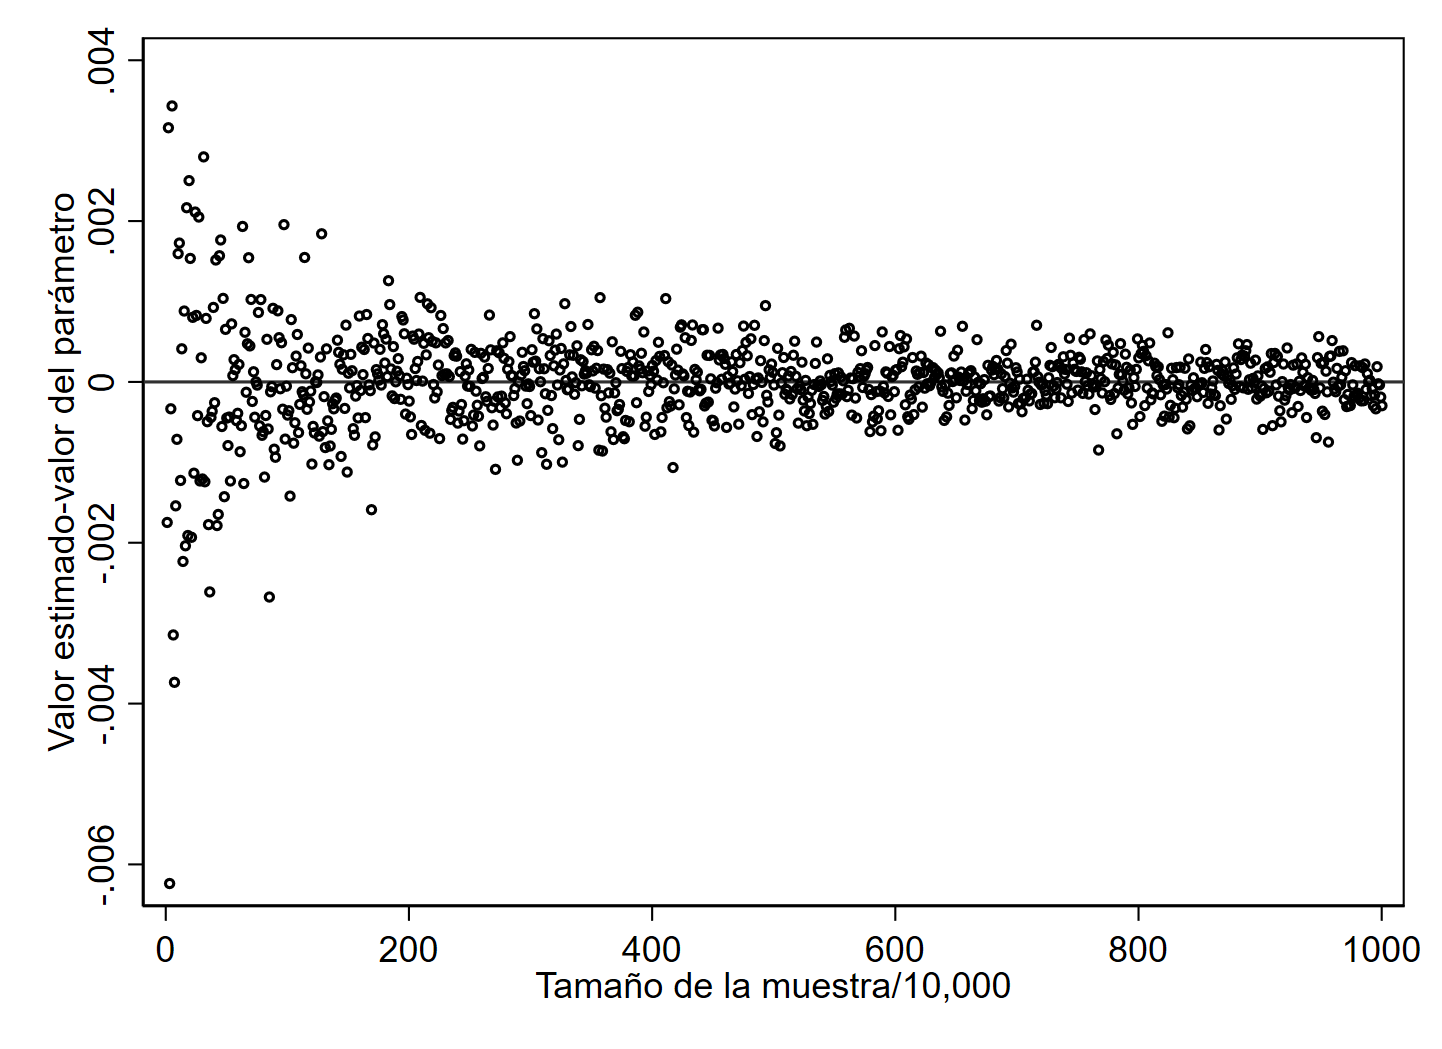
\includegraphics[width=10cm]{Figuras/convergencia-insesgamiento-estimador.png}	
\end{figure}	
\end{frame}


\begin{frame}[plain]
\begin{tcolorbox}[colback=white, arc=0mm,boxrule=0.5pt, title=Teorema del mapeo continuo (convergencia en probabilidad), breakable]	
    Sea $\textbf{g}:\RK{K} \rightarrow \RK{J}$ una función continua. Sea $\{\hat{\thetaB}_N: N=1,2,\ldots\}$ una secuencia de vectores aleatorios de $K \times 1$ tal que $\hat{\thetaB}_N \xrightarrow{p}\thetaB$, entonces $\textbf{g}(\hat{\thetaB}_N)\xrightarrow{p} \textbf{g}(\thetaB)$. \vspace{0.3cm}
\end{tcolorbox}
    %\pause
\begin{itemize}
    \item \textbf{Intuición}: Las convergencias se preservan al aplicar funciones continuas, lineales y no lineales: 
    \[
    \plim \textbf{g}(\hat{\thetaB}_N) = \textbf{g}(\plim \hat{\thetaB}_N) = \textbf{g}(\thetaB).
    \]
    %\pause
    \item \begin{Ejemplo}
    Suponga que $\hat{\theta}_N \xrightarrow{p}\theta \in \RK{+}$, y que estamos interesados en $\plim  \exp ( \hat{\theta}_N)$:
    \begin{equation*}
        \plim  \exp ( \hat{\theta}_N) =  \exp ( \plim \hat{\theta}_N) = \exp ( \theta).
    \end{equation*}        
    \end{Ejemplo}
\end{itemize}
\end{frame}


\begin{frame}[plain]
\begin{tcolorbox}[colback=white, arc=0mm,boxrule=0.5pt, title=Ley débil de los grandes números (WLLN), breakable]	
    Sea $\{\XB_i: i=1,2,\ldots, N\}$ una secuencia de vectores aleatorios de $K\times 1$ que son independientes e idénticamente distribuidos (i.i.d.) tal que $\EX \lVert \XB_i \rVert < \infty$. Entonces, se cumple la \textcolor{blue}{ley débil de los grandes números}:
    \begin{align*}
        \bar{\XB}_N = \frac{1}{N}\sum_{i=1}^{N} \XB_i \xrightarrow{p} \EX[\XB_i].
    \end{align*}
\end{tcolorbox}	
    %\pause
\begin{itemize}	
    \item \textbf{Intuición:} La media muestral converge a la media poblacional cuando $N \to \infty$. 
    \item \textbf{Nota:} Existen versiones más generales del teorema que relajan el supuesto de i.i.d. 
\end{itemize}	  
\end{frame}


\begin{frame}{Ejemplo de la ley débil de los grandes números}
\begin{itemize}
    \item Queremos estimar la \textbf{favorabilidad promedio} de un candidato antes de una elección. Seleccionamos una muestra aleatoria de \(N\) individuos y les preguntamos si apoyan al candidato (\(Y_i \in \{0, 1\}\)). %\pause 
    \vspace{0.75em}
    \begin{figure}[H]
    \centering
    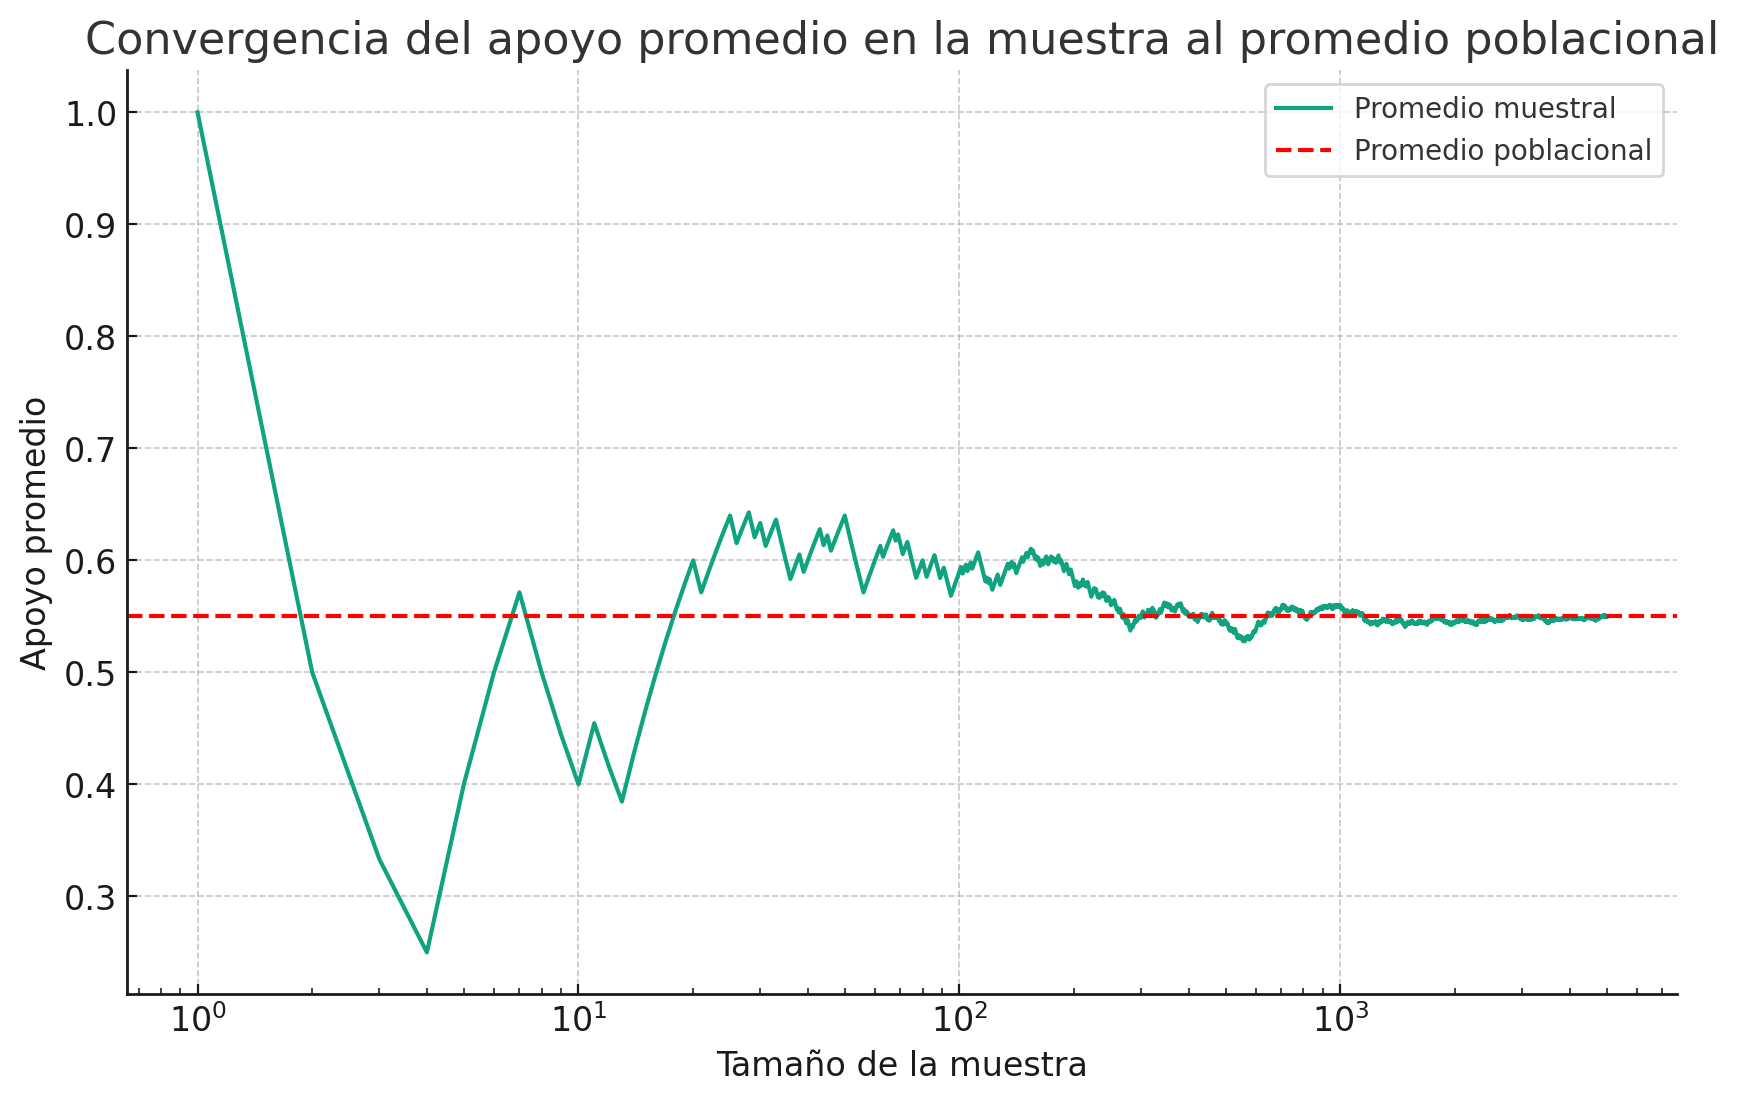
\includegraphics[width=9.5cm]{Figuras/ley-debil-grandes-numeros-encuesta.png}	
    \end{figure}	
\end{itemize}
\end{frame}


\begin{frame}{Consistencia del estimador de MCO}
\begin{itemize}
    \item Modelo lineal (proyección poblacional):
    \begin{align}\label{EQ:MODELO-LINEAL}
        Y_i = \XB'_i \textcolor{brown}{\betaB} + e_i, \quad \text{donde} \quad  \textcolor{brown}{\betaB} = \EX[\XB_i\XB'_i]^{-1} \EX[\XB_iY_i]     
    \end{align}
    \item Con una muestra aleatoria \(\{(Y_i, \XB_i): i=1,\ldots,N\}\), el estimador de MCO es:
    \vspace{-1em}
    \begin{align}\label{EQ:ESTIMADOR-MCO}
        \textcolor{brown}{\hat{\betaB}_{mco}} = \left(\frac{1}{N} \sum_i \XB_i \XB'_i \right)^{-1} \left(\frac{1}{N} \sum_i  \XB_i Y_i\right).
    \end{align}
    %\pause
    \item \textbf{Probabilidad límite}:
	\begin{align*}
	\begin{split}
	\plim \brown{\betaBH_{mco}} &= \plim \left(\textcolor{blue}{\left(\frac{1}{N}\sum_{i=1}^{N}\XB_i \XB'_i \right)^{-1}} \textcolor{red}{\left(\frac{1}{N}\sum_{i=1}^{N}\XB_i Y_i \right)}\right) \\
	&= \plim \textcolor{blue}{\left(\frac{1}{N}\sum_{i=1}^{N}\XB_i \XB'_i \right)^{-1}} \plim \textcolor{red}{\left(\frac{1}{N}\sum_{i=1}^{N}\XB_i Y_i \right) \quad \text{\small \color{brown} (mapeo cont.)}}
	\end{split}
	\end{align*} 
\end{itemize}
\end{frame}


\begin{frame}{Consistencia del estimador de MCO II}
\begin{itemize}
    \item \textbf{Primer término:} 
    \begin{align*}
    \begin{split}
        \plim \textcolor{blue}{\left(\frac{1}{N}\sum_{i=1}^{N}\XB_i \XB'_i \right)^{-1}} &= \textcolor{blue}{\left(\textcolor{black}{\plim} \frac{1}{N}\sum_{i=1}^{N}\XB_i \XB'_i \right)^{-1}} \quad \quad \text{\color{brown} (mapeo continuo)} \\ &= \EX\left[\XB_i \XB'_i\right]^{-1} \hspace{2.3cm} \text{\color{brown} (WLLN)} 
    \end{split}
    \end{align*}
    %\pause
    \item \textbf{Segundo término:}    
    \begin{align*}
    \begin{split}
        \plim \textcolor{red}{\left(\frac{1}{N}\sum_{i=1}^{N}\XB_i Y_i \right)} = \EX\left[\XB_i Y_i\right] \hspace{3cm} \text{\color{brown} (WLLN)}
    \end{split}
    \end{align*}
    %\pause
    \item \textbf{Combinando:}
    \begin{align*}
        \plim \brown{\betaBH_{mco}} = \EX[\XB_i\XB'_i]^{-1} \EX[\XB_iY_i] = \textcolor{brown}{\betaB} 
    \end{align*}
\end{itemize}
\end{frame}

%%%%%%%%%%%%%%%%%%%%%%%%%%%%%%%%%%%%%%%%%%%%%%%%%%%%%%%%%%%%%%%%%%%%%
%%%%%%%%%%%%%%%%%%%%%%%%%%%%%%%%%%%%%%%%%%%%%%%%%%%%%%%%%%%%%%%%%%%%%
\subsection{- Distribución asintótica}

\begin{frame}[plain]
\begin{tcolorbox}[colback=white, arc=0mm,boxrule=0.5pt, title=Definición: Convergencia en distribución, breakable]
    Una secuencia de variables aleatorias 
    \(\{X_N : N=1,2,\ldots\}\) 
    \textcolor{blue}{converge en distribución} a una \textbf{variable aleatoria} \(Z\) si, para todo \(x \in \mathbb{R}\) en los puntos de continuidad de la CDF de \(Z\),
    \[
        \lim_{N \to \infty} \textbf{F}_N(x) = \textbf{G}(x),
    \]
    donde 
    \[
        \textbf{F}_N(x) = \Prob{X_N \leq x} \quad \text{es la CDF de } X_N,
    \]
    y 
    \[
        \textbf{G}(x) = \Prob{Z \leq x} \quad \text{es la CDF de } Z.
    \]
\end{tcolorbox}
    %\pause
\begin{itemize}
    \item \textbf{Notación:} $X_N \xrightarrow{d} Z$ (distribución límite).	
\end{itemize}
\end{frame}


\begin{frame}[plain]
\begin{itemize}
    \item \textbf{Vectores:} La convergencia marginal de $\mathbf{X}_N$ \textcolor{red}{no implica} convergencia conjunta; la \textbf{dependencia} entre componentes importa. %\pause
    \vspace{0.75em}
\begin{tcolorbox}[colback=white, arc=0mm, boxrule=0.5pt, 
    title=\textbf{Definición: Convergencia en distribución (vectores)}, breakable]
    Una secuencia de \textbf{vectores aleatorios} 
    \(\{\XB_N : N=1,2,\ldots\}\), con dimensión \(K \times 1\), 
    \textcolor{blue}{converge en distribución} a un vector aleatorio \(\ZB \in \mathbb{R}^{K}\) si, 
    para todo vector determinístico \(\mathbf{c} \in \mathbb{R}^K\),
    \[
        \mathbf{c}' \XB_N \xrightarrow{d} \mathbf{c}' \ZB.
    \]
\end{tcolorbox}
    %\pause
    \item \textbf{Intuición:} toda combinación lineal de \(\XB_N\) converge en distribución 
    a la combinación lineal correspondiente de \(\ZB\). Esta caracterización se conoce como el \textcolor{blue}{dispositivo de Cramér--Wold}.
\end{itemize}
\end{frame}


\begin{frame}[plain]
\begin{tcolorbox}[colback=white, arc=0mm, boxrule=0.5pt, 
    title=\textbf{Teorema del mapeo continuo (convergencia en distribución)}, breakable]
    Sea \(\{\hat{\thetaB}_N : N=1,2,\ldots\}\) una secuencia de vectores aleatorios 
    de dimensión \(K \times 1\) tal que 
    \vspace{-1em}
    \[
        \hat{\thetaB}_N \xrightarrow{d} \ZB.
    \]
    
    \vspace{-0.75em}
    Si \(\mathbf{g}: \mathbb{R}^K \to \mathbb{R}^J\) es una función continua, entonces
    \vspace{-0.75em}
    \[
        \mathbf{g}(\hat{\thetaB}_N) \xrightarrow{d} \mathbf{g}(\ZB).
    \]
\end{tcolorbox}
    %\pause
\begin{itemize}
    \item \textbf{Intuición:} Si conocemos la distribución límite de \(\hat{\thetaB}_N\), también conocemos la distribución límite de cualquier función continua de \(\hat{\thetaB}_N\).
\end{itemize}
\end{frame}


\begin{frame}[plain]
\begin{tcolorbox}[colback=white, arc=0mm, boxrule=0.5pt, 
    title=\textbf{Teorema del límite central (CLT) – Lindeberg–Lévy}, breakable]
    Sea \(\{\XB_i : i=1,2,\ldots,N\}\) una secuencia de vectores aleatorios 
    de dimensión \(K \times 1\), independientes e idénticamente distribuidos (i.i.d.), 
    con media finita \(\EX[\XB_i] = \boldsymbol{\mu}\) y matriz de covarianza finita 
    \(\Sigma = \EX[(\XB_i - \boldsymbol{\mu})(\XB_i - \boldsymbol{\mu})']\). Entonces,
    \[
        \sqrt{N}\,(\bar{\XB}_N - \boldsymbol{\mu}) \xrightarrow{d} \mathcal{N}(\textbf{0},\Sigma),
    \]
    donde \(\bar{\XB}_N = \tfrac{1}{N}\sum_{i=1}^{N}\XB_i\).
\end{tcolorbox}
 %\pause
\begin{itemize}
    \item \textbf{Nota:} Existen versiones más generales del teorema que relajan el supuesto de i.i.d. (e.g., dependencia débil, heterogeneidad limitada). %\pause
    \item No se asume normalidad de $\mathbf{X}_i$; la normalidad emerge en el promedio. %\pause
    \item Un estimador tiene una \textcolor{blue}{tasa de convergencia} a raíz-$N$ si el error estándar del estimador disminuye proporcionalmente a $1/\sqrt{N}$.
\end{itemize}
\end{frame}


\begin{frame}{Simulación del teorema del límite central}
\begin{itemize}
    \item \textbf{Distribuciones consideradas:}
    \vspace{0.5em}
    \begin{itemize}
        \item[i.] \(\textbf{f}(x) = \lambda \exp(-\lambda x)\), con \(\lambda=1\) \hfill (\textcolor{brown}{Exponencial})
              \vspace{0.2cm}
        \item[ii.] \(\textbf{f}(x) = 1/(b-a)\), con \(a=0, b=1\) \hfill (\textcolor{brown}{Uniforme}) 
              \vspace{0.2cm}
        \item[iii.] \(X \sim \text{\textbf{Bernoulli}}(p)\), con \(p=0.5\) \hfill (\textcolor{brown}{Bernoulli})
              \vspace{0.3cm}
    \end{itemize}    
    %\pause
    \item \textbf{Algoritmo (repetido 10,000 veces):}
    \begin{enumerate}
        \item Extraer una muestra i.i.d. de tamaño \(N=10^5\) de cada distribución.
        \item Calcular el promedio muestral \(\bar{X}_N\).
        \item Estandarizar:  
              \[
                  Z_N = \frac{\sqrt{N}\,(\bar{X}_N - \mu)}{\sigma}.
              \]
        \item Guardar \(\bar{X}_N\) y \(Z_N\) para cada muestra y distribución.
    \end{enumerate}
\end{itemize}
\end{frame}


\begin{frame}{Resultados simulación: distribución de $Z_N$}
\vspace{-0.3cm}				
\begin{figure}[H]
	\begin{subfigure}{.49\textwidth}
		\caption{Exponencial}	
		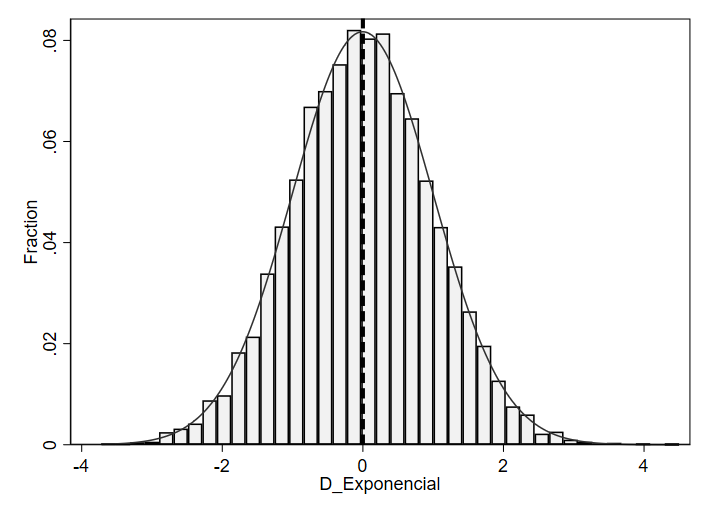
\includegraphics[width=4.5cm, height=4.5cm, keepaspectratio]{Figuras/clt-simulacion-zn-exponencial.png}
	\end{subfigure}
	\begin{subfigure}{.49\textwidth}
		\caption{Uniforme}
		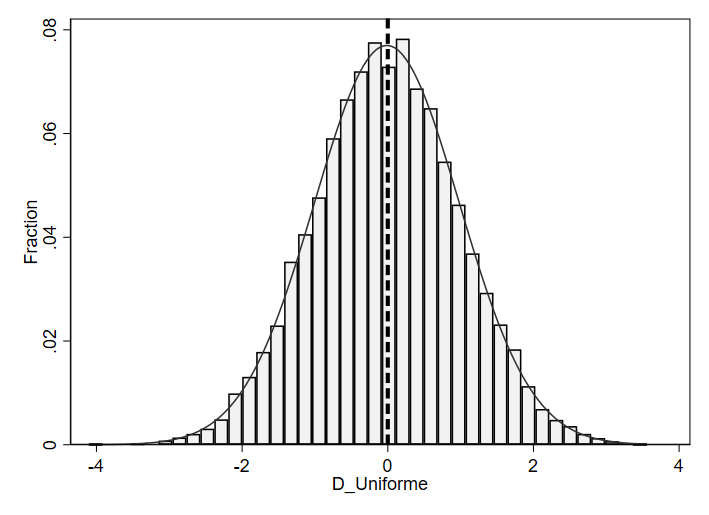
\includegraphics[width=4.5cm, height=4.5cm, keepaspectratio]{Figuras/clt-simulacion-zn-uniforme.png}
	\end{subfigure}	
    \begin{subfigure}{.49\textwidth}
        \caption{Bernoulli}	
		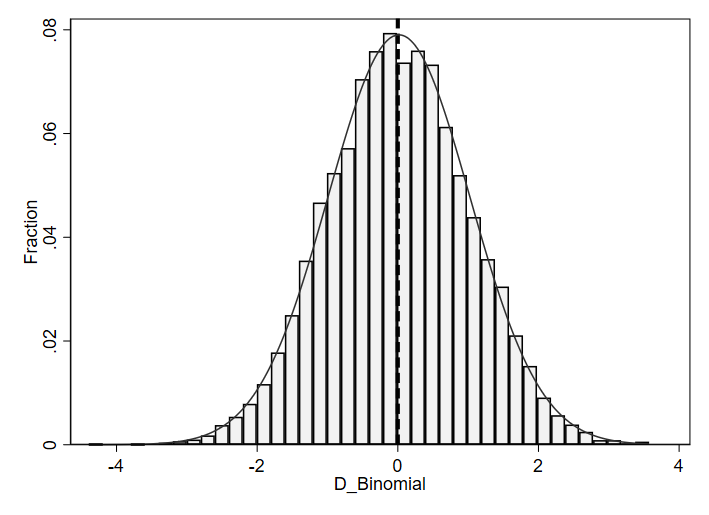
\includegraphics[width=4.5cm, height=4.5cm, keepaspectratio]{Figuras/clt-simulacion-zn-bernoulli.png}
	\end{subfigure}		
\end{figure}	
\end{frame}

\begin{frame}{Convergencia en distribución y convergencia en probabilidad}
\begin{itemize}
    \item Queremos estimar la \textbf{favorabilidad promedio} de un candidato antes de una elección. Seleccionamos una muestra aleatoria de \(N\) individuos y les preguntamos si apoyan al candidato (\(Y_i \in \{0, 1\}\)).  
    \vspace{0.5cm}
       %\pause
\begin{figure}[H]
	\centering
	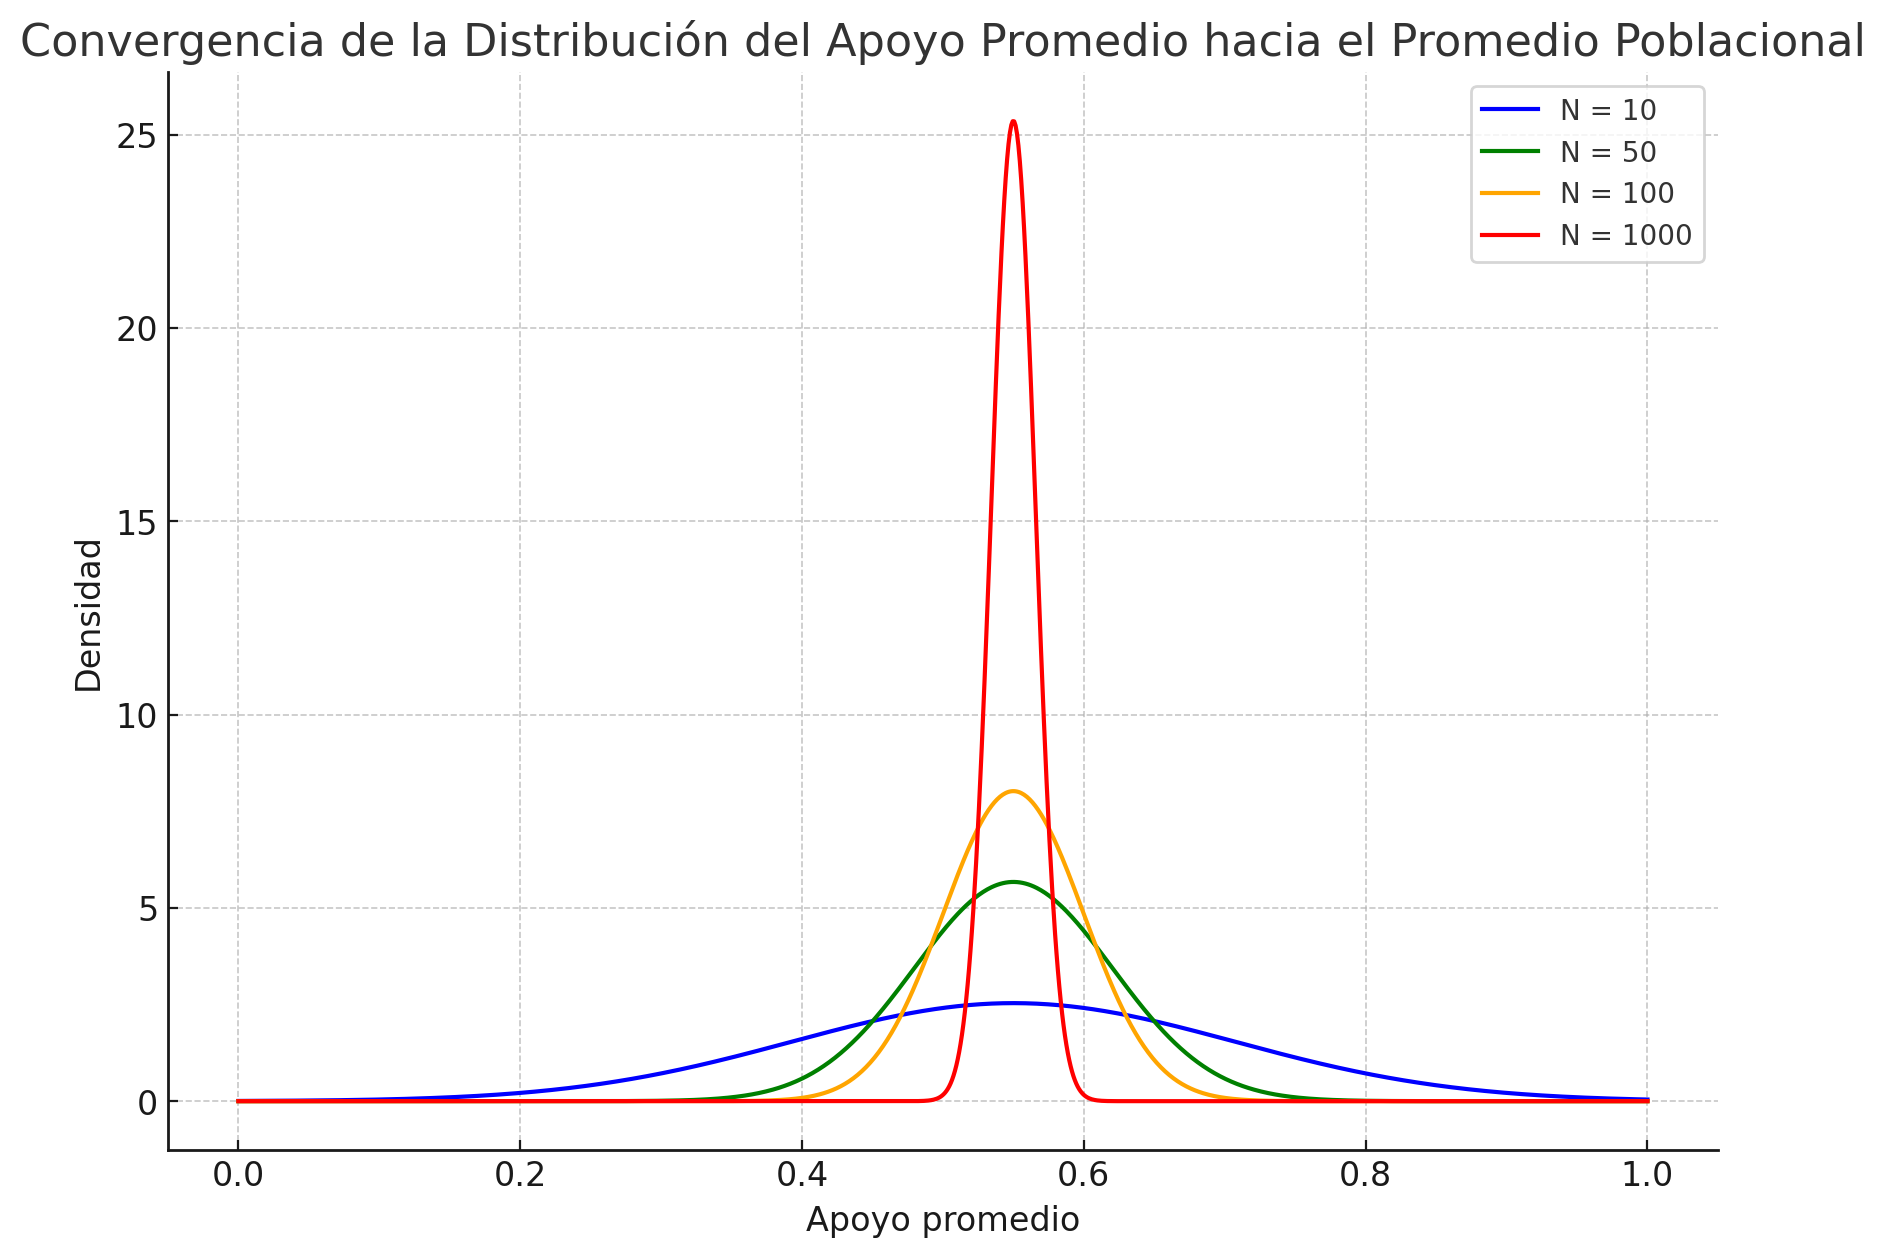
\includegraphics[width=9cm]{Figuras/teorema-central-limite-encuesta.png}	
\end{figure}	
\end{itemize}
\end{frame}

\begin{frame}{Distribución asintótica del estimador de MCO}
\begin{itemize}
    \item Muestra aleatoria: \(\{(Y_i, \XB_i): i=1,\ldots,N\}\).
    \[
        \brown{\betaBH_{mco}} 
        = \Bigg(\frac{1}{N}\sum_{i=1}^{N}\XB_i \XB'_i \Bigg)^{-1} 
          \Bigg(\frac{1}{N}\sum_{i=1}^{N}\XB_i Y_i \Bigg).
    \]
    
    %\pause
    \item Sustituyendo \(Y_i = \XB'_i \textcolor{brown}{\betaB} + e_i\):
    \[
        \brown{\betaBH_{mco}} 
        = \brown{\betaB} 
          + \Bigg(\frac{1}{N}\sum_{i=1}^{N}\XB_i \XB'_i \Bigg)^{-1} 
            \Bigg(\frac{1}{N}\sum_{i=1}^{N}\XB_i e_i \Bigg).
    \]
    
    %\pause
    \item Reorganizando y multiplicando por \(\sqrt{N}\):
    \[
        \sqrt{N}\,\big(\brown{\betaBH_{mco}} - \brown{\betaB}\big) 
        = \Bigg(\frac{1}{N}\sum_{i=1}^{N}\XB_i \XB'_i \Bigg)^{-1}
        \underbrace{\Bigg(\frac{1}{\sqrt{N}}\sum_{i=1}^{N}\XB_i e_i \Bigg)}_{\textcolor{olive}{\text{término estocástico}}}.
    \]
\end{itemize}
\end{frame}


\begin{frame}{Distribución del término estocástico}
\begin{itemize}
    \item Definamos \(\WB_i \equiv \XB_i e_i\) y su promedio muestral \(\bar{\WB}_N = \frac{1}{N}\sum_{i=1}^N \WB_i\).    
    %\pause
    \vspace{0.5em}
    \item Por la \textcolor{blue}{ley de los grandes números}:
    \[
        \plim \bar{\WB}_N = \EX[\WB_i] = \EX[\XB_i e_i] = \textbf{0}.
    \]   
    %\pause
    \item Consideremos la suma:
    \(
        \frac{1}{\sqrt{N}}\sum_{i=1}^{N}\WB_i 
        = \sqrt{N}\,\bar{\WB}_N.
    \)
    \vspace{0.5em}
    %\pause
    \item Por el \textcolor{blue}{teorema del límite central (CLT)}:
    \[
        \sqrt{N}\,\bar{\WB}_N \xrightarrow{d} \mathcal{N}(\textbf{0},\Sigma),
    \]
    donde \(\Sigma = \Var(\WB_i) = \EX[\WB_i \WB_i'] = \EX\Big[(\XB_i e_i) (\XB_i e_i)'\Big] = \EX[\XB_i \XB'_i e^2_i]\).
\end{itemize}
\end{frame}


\begin{frame}[plain]
\begin{tcolorbox}[colback=white, arc=0mm, boxrule=0.5pt, 
    title=\textbf{Teorema de Slutsky (corolario)}, breakable]

    Si 
    \[
        \sqrt{N}\,\bar{\WB}_N \xrightarrow{d} \mathcal{N}(\textbf{0}, \Sigma),
    \]
    y 
    \[
        \AB_N \xrightarrow{p} \AB,
    \]
    entonces
    \[
        \AB_N \,\sqrt{N}\,\bar{\WB}_N \xrightarrow{d} \mathcal{N}\!\left(\textbf{0},\, \AB \Sigma \AB' \right).
    \]
\end{tcolorbox}	
\begin{itemize}
    %\pause
    \item En nuestro caso particular:
    \[
        \textbf{A}_N \equiv \Bigg(\frac{1}{N}\sum_{i=1}^{N}\XB_i \XB'_i \Bigg)^{-1} \xrightarrow{p} \EX\left[\XB_i \XB'_i\right]^{-1} \equiv \textbf{A}. \hspace{0.75cm} \text{\color{brown} (WLLN)} 
    \]
\end{itemize}
\end{frame}


\begin{frame}{Distribución límite de $\sqrt{N}\,\big(\brown{\betaBH_{mco}} - \brown{\betaB}\big)$}
\begin{itemize}
    \item En resumen, hemos mostrado que:
    \begin{align}\label{EQ:CONVDIST-MCO}
    \begin{split}
    \sqrt{N}\,\big(\brown{\betaBH_{mco}} - \brown{\betaB}\big) = \AB_N \,\sqrt{N}\,\bar{\WB}_N \xrightarrow{d} \mathcal{N}\!\left(\textbf{0},\, \AB \Sigma \AB' \right)       
    \end{split}
    \end{align}
     donde:
    \begin{itemize}
        \item \(\AB = \EX[\XB_i \XB_i']^{-1}\),
        \item \(\Sigma = \EX[\XB_i \XB_i' e_i^2]\).
    \end{itemize}
    %\pause
    \vspace{1em}
    \item Por lo tanto, la \textbf{matriz de varianza-covarianza} de \(K \times K\) es
    \begin{align}\label{EQ:VARCOV}     
    \AB \Sigma \AB' 
    = \EX[\XB_i \XB_i']^{-1} 
      \,\EX[\XB_i \XB_i' e_i^2]\,
      \EX[\XB_i \XB_i']^{-1}.
    \end{align}
    %\pause
    Los errores estándar teóricos utilizados para construir los estadísticos de prueba son las raíces cuadradas de los elementos diagonales de \(\tfrac{1}{N}\AB \Sigma \AB'\), es decir, de la ecuación \eqref{EQ:VARCOV} dividida por \(N\).
\end{itemize}
\end{frame}


\begin{frame}{Distribución asintótica del estimador de MCO}
\begin{itemize}
    \item Para obtener la distribución (aproximada) del estimador, dividimos por $\sqrt{N}$ y sumamos $\brown{\betaB}$. \vspace{-1em}
    \begin{align*}
    \begin{split}
        \brown{\betaBH_{mco}} \distras{a} \mathcal{N}(\brown{\betaB}, \frac{1}{N} \AB \Sigma \AB').
    \end{split}
    \end{align*}	
 %\pause
    La llamamos \textcolor{blue}{distribución asintótica}. Esta es una \textcolor{red}{aproximación para muestras finitas pero ``suficientemente'' grandes}. \vspace{1em}
 %\pause
    \item Recordar que $\brown{\betaBH_{mco}} \xrightarrow{p} \brown{\betaB}$, y el parámetro $\brown{\betaB}$ no es estocástico, así que la distribución límite de $\brown{\betaBH_{mco}}$ es degenerada.     
\end{itemize}
\end{frame}


%%%%%%%%%%%%%%%%%%%%%%%%%%%%%%%%%%%%%%%%%%%%%%%%%%%%%%%%%%%%%%%%%%%%%
%%%%%%%%%%%%%%%%%%%%%%%%%%%%%%%%%%%%%%%%%%%%%%%%%%%%%%%%%%%%%%%%%%%%%
\subsection{- Errores estándar del estimador de MCO}

\begin{frame}{Estimadores de la matriz de varianza--covarianza ($\AB \Sigma \AB'$)}
\begin{itemize}
    \item La matriz de varianza--covarianza depende de momentos poblacionales que en la práctica debemos \textcolor{blue}{estimar}. \pause
    \vspace{1em}
    \item La elección del estimador depende de los \textcolor{blue}{supuestos} que hagamos sobre el término de error \(e_i\) en el modelo. \pause
    \vspace{1em}
    \item Tres casos frecuentes en econometría aplicada:
    \vspace{0.5em}
    \begin{enumerate}
        \item \textbf{Homoscedasticidad y no autocorrelación}: Supuesto clásico de MCO, pero \textcolor{red}{MUY} restrictivo. \pause
        \item \textbf{Heteroscedasticidad y no autocorrelación}: Errores estándar \textit{robustos} de White. \pause
        \item \textbf{Heteroscedasticidad con autocorrelación en grupos}:  Errores estándar agrupados o \emph{clustered}. \pause
    \end{enumerate}
    \vspace{0.5em}
    \item En cada caso, usamos los residuos estimados: \(\hat{e}_i = Y_i - \XB'_i \brown{\betaBH_{mco}}\).
 \end{itemize}
\end{frame}


\begin{frame}{Homoscedasticidad y no autocorrelación}\label{DIAP:estVarCons}
\begin{itemize}
    \item \textbf{Supuestos:}
    \vspace{-0.75em}
    \[
    \EX[e_i^2 \mid \XB] = \brown{\sigma^2} \;\; \forall i, \quad \text{y} \quad \EX[e_i e_j \mid \XB] = 0 \;\; \text{para} \;\; i \neq j.
    \]
    \pause
    \item En este caso,
    \vspace{-0.75em}
    \begin{align*}
    \begin{split}
        \AB \Sigma \AB' &= \EX[\XB_i \XB_i']^{-1} \EX\Big[\XB_i \XB_i' \EX[e_i^2 \mid \XB_i]\Big] \EX[\XB_i \XB_i']^{-1} \quad \quad (\textcolor{brown}{\text{LEI}}) \\
        &= \brown{\sigma^2} \EX[\XB_i \XB_i']^{-1}
    \end{split}
    \end{align*}
    \pause
    \item Si definimos \(\brown{\hat{\sigma}^2} = \frac{\sum_{i}\hat{e}^2_i}{N-K}\), se puede \hyperlink{ANEX:estVarCons}{{\beamerreturnbutton{demostrar}}} que
    \vspace{-0.5em}
    \begin{align*}
    \begin{split}
        \plim \brown{\hat{\sigma}^2} = \brown{\sigma^2}.
    \end{split}
    \end{align*}
    \pause
    \vspace{-0.75em}
    Así, se cumple: 
    \[
        \plim \brown{\hat{\sigma}^2} \left(\frac{1}{N}\sum_{i=1}^{N}\XB_i \XB'_i \right)^{-1} = \AB \Sigma \AB'.
    \]
 \end{itemize}
\end{frame}


\begin{frame}{Heteroscedasticidad y no autocorrelación}
\begin{itemize}
    \item \textbf{Supuestos:}
    \vspace{-0.75em}
    \[
    \EX[e_i^2 \mid \XB] = \brown{\sigma^2_i}, \quad \text{y} \quad \EX[e_i e_j \mid \XB] = 0 \;\; \text{para} \;\; i \neq j.
    \]
    \pause
    \item \citet{white1980} demuestra que
    \begin{align*}
    \begin{split}
        \plim \frac{1}{N} \sum_{i=1}^{N} \XB_i \XB'_i \hat{e}^2_i = \EX[\XB_i \XB_i' e_i^2].
    \end{split}
    \end{align*}
    \vspace{0.5em}
    \pause
    Por consiguiente, se cumple:
    \begin{align*}
        \plim \underbrace{\left(\frac{1}{N}\sum_{i=1}^{N}\XB_i \XB'_i \right)^{-1}}_{\textbf{A}_N} \underbrace{\frac{1}{N} \sum_{i=1}^{N} \XB_i \XB'_i \hat{e}^2_i}_{\hat{\Sigma}} \underbrace{\left(\frac{1}{N}\sum_{i=1}^{N}\XB_i \XB'_i \right)^{-1}}_{\textbf{A}_N}  = \AB \Sigma \AB'        
    \end{align*}
 \end{itemize}
\end{frame}


\begin{frame}{Modelo con heteroscedasticidad}
    \begin{figure}[H]
    \centering
    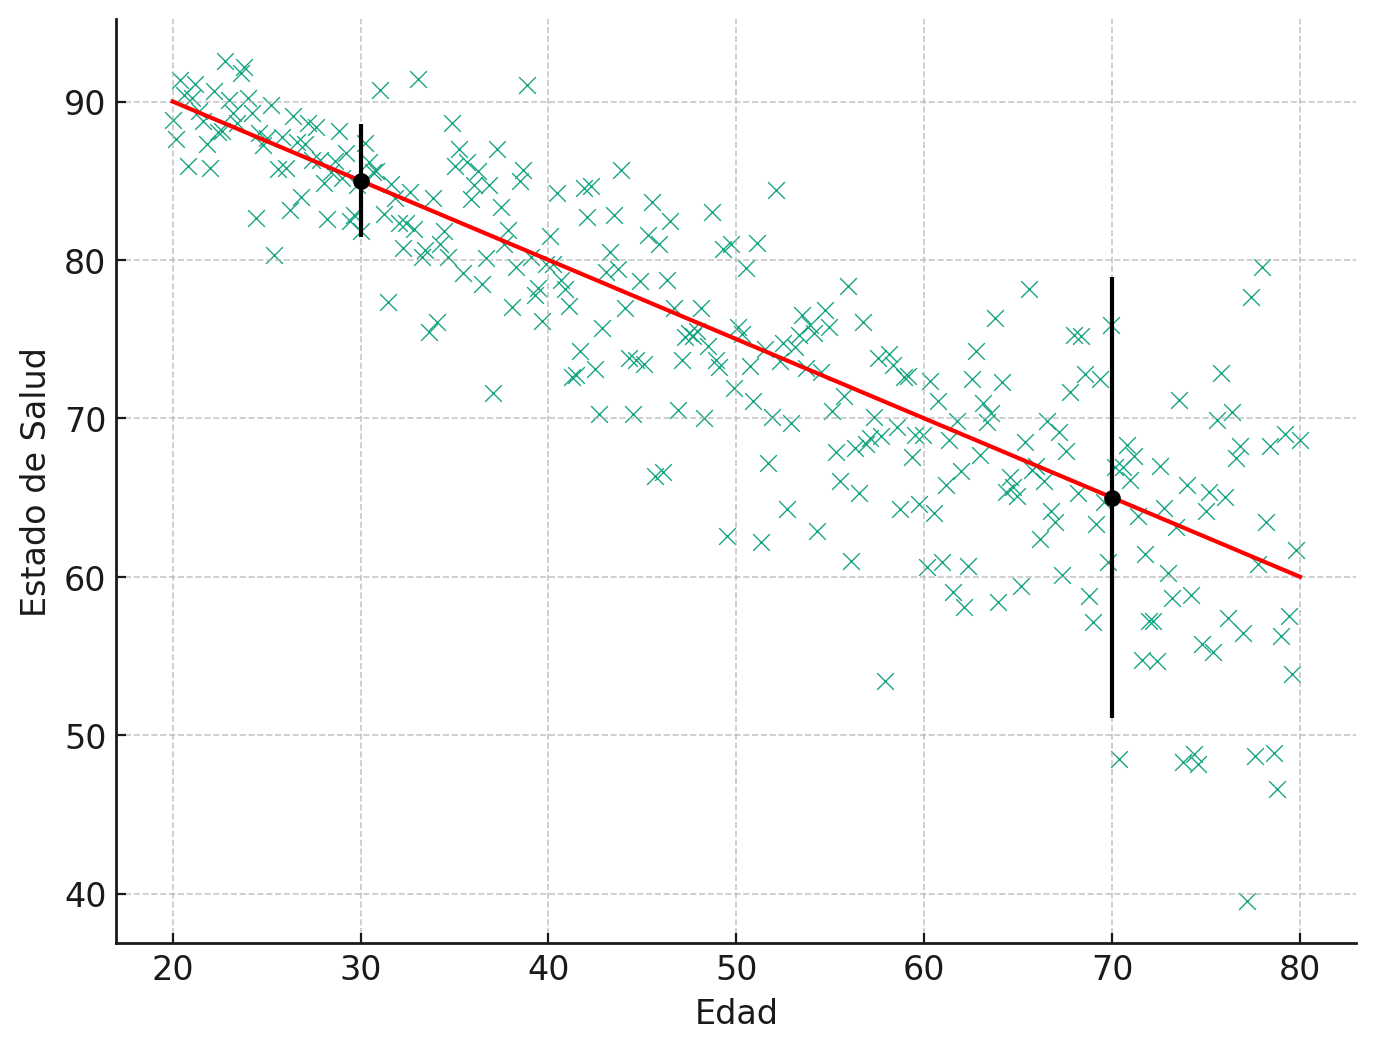
\includegraphics[width=8.5cm]{Figuras/modelo-regresion-heterocedasticidad.png}	
\end{figure}    
\end{frame}


\begin{frame}{Heteroscedasticidad con autocorrelación en grupos}
\begin{itemize}
    \item Dividimos las \(N\) observaciones en grupos \(g \in \{1, \ldots, G\}\). \pause
    \vspace{0.5em}
    \item \textbf{Supuestos:}
    \vspace{-1.3em}
    \begin{align*}
    \footnotesize
    \begin{split}
    \EX[e_{gi}^2 \mid \XB] &= \sigma^2_{gi}, \\
    \EX[e_{gi} e_{gj} \mid \XB] &\;\;\text{no se restringe} \quad \text{si } i \neq j, \\
    \EX[e_{gi} e_{hj} \mid \XB] &= 0 \quad \text{si } g \neq h.
    \end{split}
    \end{align*}
    Es decir, se permite \textbf{heteroscedasticidad y correlación arbitraria dentro de cada grupo}, pero independencia entre grupos. \pause
    \vspace{0.5em}
    \item Si definimos:
    \vspace{-1em}
    \begin{align*}    
    \footnotesize
        \hat{\Sigma} \equiv \frac{1}{N} \sum_{g=1}^{G} \left( \sum_{i \in g} \XB_{gi}\hat{e}_{gi} \right)
        \left( \sum_{i \in g} \XB_{gi}\hat{e}_{gi} \right)',
    \end{align*}
    \vspace{-0.25em}
    \pause
    se cumple:
    \vspace{-1em}
    \begin{align*}
    \footnotesize
        \plim \underbrace{\left(\frac{1}{N}\sum_{i=1}^{N} \XB_i \XB'_i \right)^{-1}}_{\textbf{A}_N}
        \hat{\Sigma}
        \underbrace{\left(\frac{1}{N}\sum_{i=1}^{N} \XB_i \XB'_i \right)^{-1}}_{\textbf{A}_N} = \AB \Sigma \AB'.
    \end{align*}
    \vspace{-0.5em}
    \item \textbf{Nota:} La consistencia de este estimador requiere que el número de grupos \(G \to \infty\).
\end{itemize}
\end{frame}

\begin{frame}{Resumiendo}
\begin{itemize}
    \item La distribución asintótica del estimador MCO es:
    \vspace{-0.5em}
    \[
        \brown{\betaBH_{mco}} \distras{a} 
        \mathcal{N}\!\left(\brown{\betaB}, \tfrac{1}{N}\AB \Sigma \AB'\right),
    \]
    donde \(\AB \Sigma \AB'\) es la matriz de varianza--covarianza que debemos estimar.
    \vspace{-0.0em}
    \pause
    \item Según los supuestos sobre el término de error, obtenemos distintos estimadores consistentes:
    \[
        \plim \, \AB_N \hat{\Sigma} \AB_N' = \AB \Sigma \AB',
    \]
    \vspace{-0.0em}    
    donde \(\AB_N\) es un estimador consistente de \(\AB\) y \(\hat{\Sigma}\) es un estimador consistente de \(\Sigma\). \pause
    \vspace{0.5em}
    \item Los errores estándar para construir los estadísticos de prueba son las raíces cuadradas de los elementos diagonales de \(\tfrac{1}{N}\AB_N \hat{\Sigma} \AB_N'\).
\end{itemize}
\end{frame}


%%%%%%%%%%%%%%%%%%%%%%%%%%%%%%%%%%%%%%%%%%%%%%%%%%%%%%%%%%%%%%%%%%%%%
%%%%%%%%%%%%%%%%%%%%%%%%%%%%%%%%%%%%%%%%%%%%%%%%%%%%%%%%%%%%%%%%%%%%%
\section{Anexos}

%%%%%%%%%%%%%%%%%%%%%%%%%%%%%%%%%%%%%%%%%%%%%%%%%%%%%%%%%%%%%%%%%%%%%
%%%%%%%%%%%%%%%%%%%%%%%%%%%%%%%%%%%%%%%%%%%%%%%%%%%%%%%%%%%%%%%%%%%%%
\subsection{- Insesgamiento}

\begin{frame}{Propiedades de los estimadores en muestras finitas}
\begin{itemize}
    \item Consideraremos dos propiedades de los estimadores en \textbf{muestras finitas}:
    \begin{enumerate}
        \item \textcolor{blue}{Insesgamiento:} Un estimador \(\textcolor{brown}{\hat{\theta}}\) del parámetro \(\textcolor{brown}{\theta}\) es insesgado si \(\EX [\textcolor{brown}{\hat{\theta}}] = \textcolor{brown}{\theta}\). 
        % %%%%%%%%\pause
        \vspace{0.2cm}        
        \item \textcolor{blue}{Eficiencia:} Sean \(\textcolor{brown}{\hat{\theta}}\) y \(\textcolor{brown}{\tilde{\theta}}\) dos estimadores insesgados del parámetro \(\textcolor{brown}{\theta}\). Decimos que \(\textcolor{brown}{\hat{\theta}}\) es más eficiente que \(\textcolor{brown}{\tilde{\theta}}\) si \( \Var[\textcolor{brown}{\hat{\theta}}] < \Var[\textcolor{brown}{\tilde{\theta}}]\).
    \end{enumerate}
\end{itemize}
\end{frame}


\begin{frame}{Insesgamiento del estimador de MCO I}
\begin{itemize}
    \item Modelo lineal (proyección poblacional):
    \begin{align}\label{EQ:MODELO-LINEAL-B}
        Y_i = \XB'_i \textcolor{brown}{\betaB} + e_i, \quad \text{donde} \quad  \textcolor{brown}{\betaB} = \EX[\XB_i\XB'_i]^{-1} \EX[\XB_iY_i]        
    \end{align}
    \item Para demostrar \textcolor{blue}{insesgamiento} y \textcolor{blue}{eficiencia}, necesitamos un supuesto más fuerte: \(\EX[e_i \mid \XB_i] = 0\) (i.e., la CEF es lineal) 
    \vspace{0.5em}
    \item Con una muestra aleatoria \(\{(Y_i, \XB_i): i=1,\ldots,N\}\), el estimador de MCO es:
    \vspace{-0.5em}
    \begin{align}\label{EQ:ESTIMADOR-MCO-B}
        \textcolor{brown}{\hat{\betaB}_{mco}} = \left(\sum_i \XB_i \XB'_i \right)^{-1} \left(\sum_i  \XB_i Y_i\right).
    \end{align}
    \vspace{-0.5em}
    % %%%%%%%%\pause
    Sustituyendo \eqref{EQ:MODELO-LINEAL-B} en \eqref{EQ:ESTIMADOR-MCO-B}:
    \begin{align*}
    \begin{split}
        \textcolor{brown}{\hat{\betaB}_{mco}} = \textcolor{brown}{\betaB} + \left(\sum_i \XB_i \XB'_i \right)^{-1} \left(\sum_i  \XB_i e_i\right)
    \end{split}
    \end{align*}
\end{itemize}
\end{frame}


\begin{frame}{Insesgamiento del estimador de MCO II}
\begin{itemize}
    \item Tomando el \textbf{valor esperado condicional en la muestra \(\XB\)}:
    \begin{align*}
        \EX[\textcolor{brown}{\hat{\betaB}_{mco}}|\XB] 
        &= \textcolor{brown}{\betaB} 
           + \EX\!\left[ 
             \Bigg(\sum_i \XB_i \XB'_i \Bigg)^{-1} 
             \Bigg(\sum_i \XB_i e_i\Bigg) \;\Bigg|\; \XB
             \right] \\
        &= \textcolor{brown}{\betaB} 
           + \Bigg(\sum_i \XB_i \XB'_i \Bigg)^{-1} 
             \Bigg(\sum_i \XB_i \EX[e_i \mid \XB]\Bigg) \\
        &= \textcolor{brown}{\betaB}.
    \end{align*}
    % %%%%%%%%\pause
    \item Usando la \textbf{ley de la esperanza iterada}:
    \begin{align*}
        \EX[\textcolor{brown}{\hat{\betaB}_{mco}}] &= \EX\left[\EX[\textcolor{brown}{\hat{\betaB}_{mco}}|\XB]\right] \\
        &= \textcolor{brown}{\betaB}.
    \end{align*}
    % %%%%%%%%\pause
    $\implies$ El \textcolor{blue}{estimador de MCO} es \textcolor{blue}{insesgado}.
\end{itemize}
\end{frame}


\begin{frame}{Ejemplo de insesgamiento en datos simulados}
\begin{itemize}
    \item \textbf{Modelo Poblacional:}
    \begin{align*}
        Y_i = \textcolor{brown}{\beta_0} + \textcolor{brown}{\beta_1} X_i + e_i
    \end{align*}
    \item \textbf{Supuestos:}
    \begin{itemize}
        \item[i.] \(\textcolor{brown}{\beta_0} = 10\), \(\textcolor{brown}{\beta_1} = 5\)
        \vspace{0.1cm}
        \item[ii.] \(X_i \sim \mathcal{N}(8, 16)\), \(e_i \sim \mathcal{N}(0, 9)\), independientes \(\Rightarrow \EX[e_i \mid X_i] = 0\)
    \end{itemize}
    \vspace{1em}
    % %%%%%%%%\pause
    \item \textbf{Algoritmo (se repite 10,000 veces):}
    \begin{enumerate}
        \item Generar una muestra aleatoria (iid) de tamaño \textcolor{red}{\(N = 100\)} para \(X_i\) y \(e_i\).
        \item Calcular \(Y_i\) usando los parámetros del modelo poblacional.
        \item Estimar los parámetros por MCO, dada la muestra: 
        \begin{align*}
            \textcolor{brown}{\hat{\betaB}_{mco}} = \left(\XB' \XB \right)^{-1} \XB' \YB
        \end{align*}
        \item Guardar los valores estimados de \(\textcolor{brown}{\hat{\beta}_0}\) y \(\textcolor{brown}{\hat{\beta}_1}\).
    \end{enumerate}
\end{itemize}
\end{frame}

\begin{frame}{Distribución de $\textcolor{brown}{\hat{\beta}_0}$, $\textcolor{brown}{\hat{\beta}_1}$ en las 10,000 simulaciones}
\begin{figure}[H]
	\begin{subfigure}{.49\textwidth}
		\caption{$\textcolor{brown}{\hat{\beta}_0}$  (promedio = 10.00)}	
		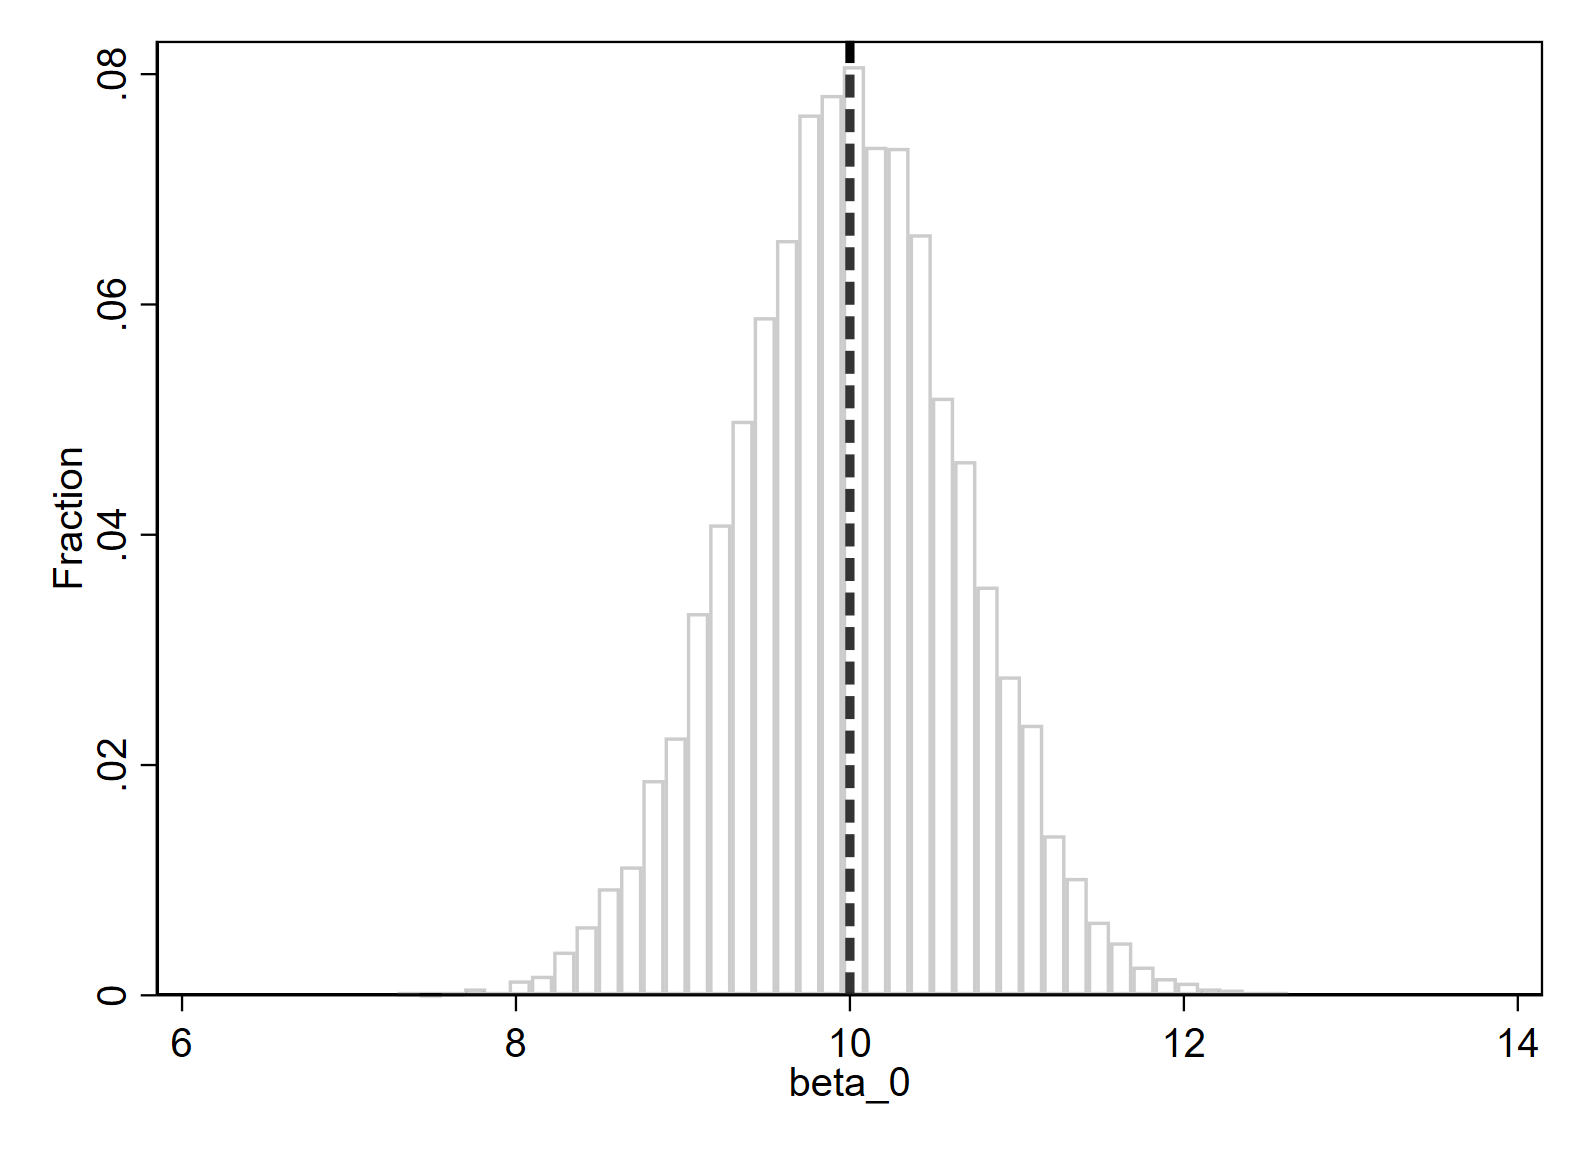
\includegraphics[width=5.5cm, height=5.5cm, keepaspectratio]{Figuras/simulacion-distribucion-beta0.png}
	\end{subfigure}
	\begin{subfigure}{.49\textwidth}
		\caption{$\textcolor{brown}{\hat{\beta}_1}$ (promedio = 4.99)}
		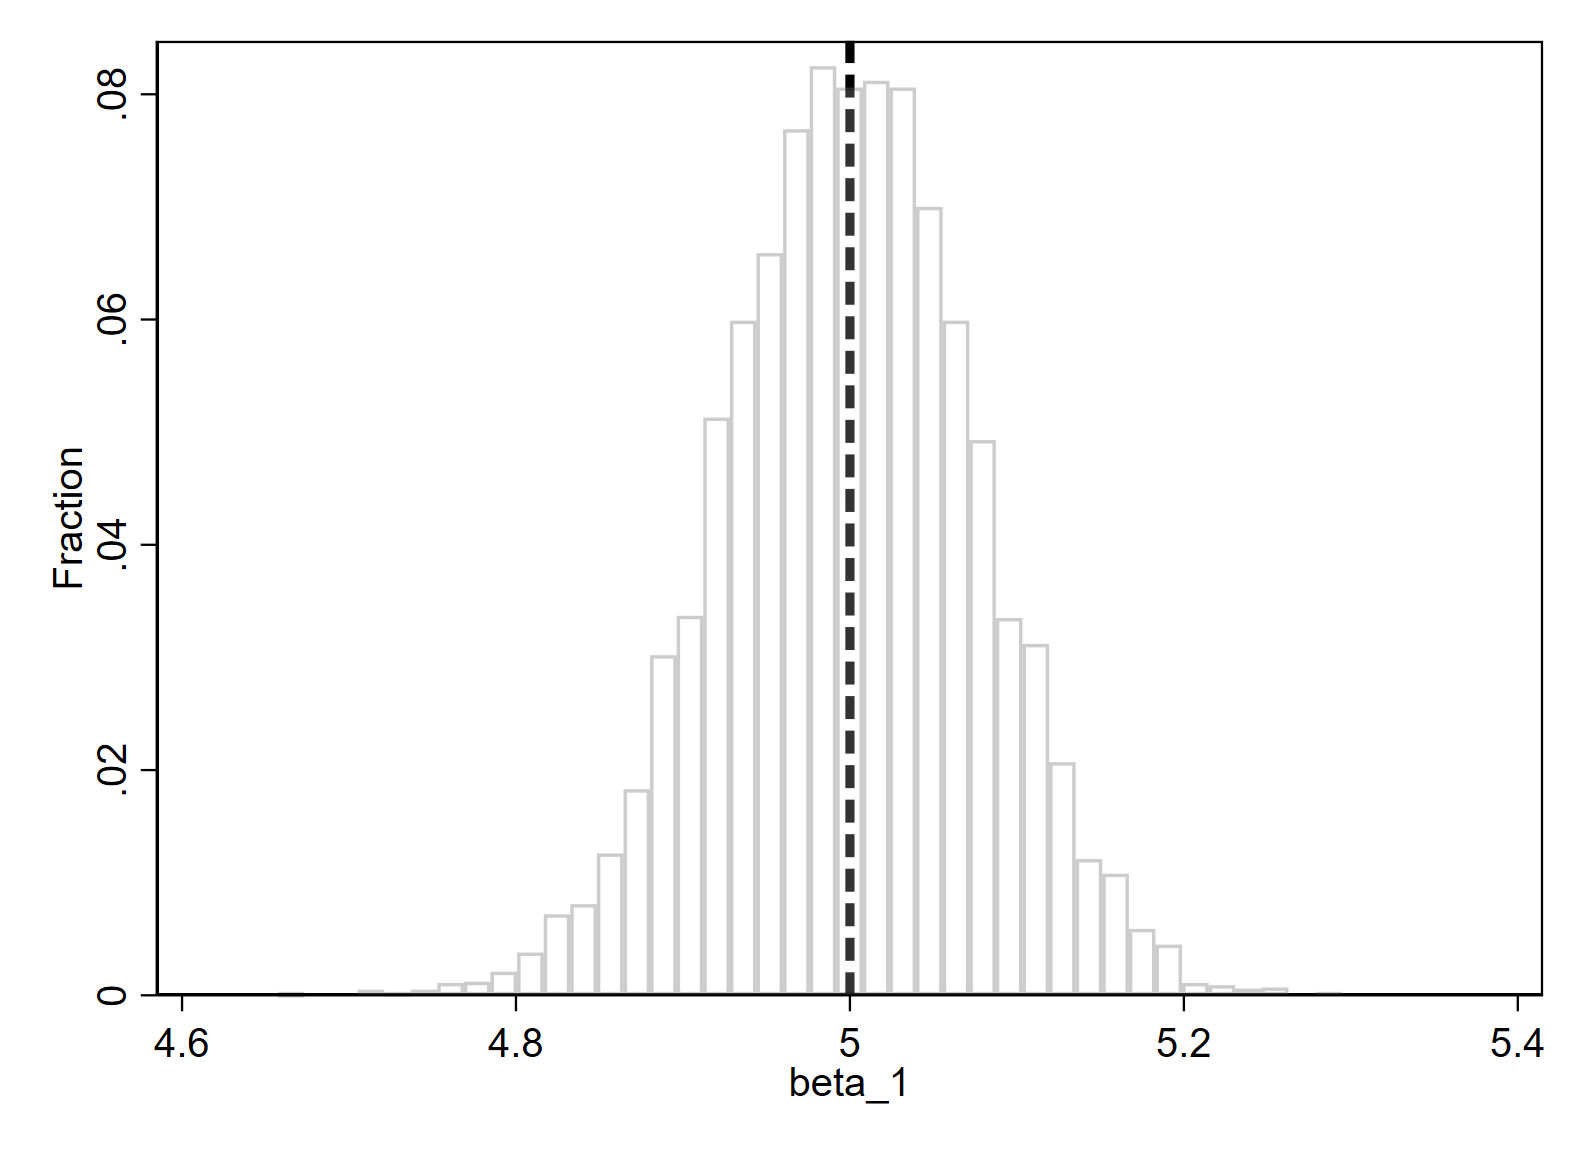
\includegraphics[width=5.5cm, height=5.5cm, keepaspectratio]{Figuras/simulacion-distribucion-beta1.png}
	\end{subfigure}	
\end{figure}	
\begin{itemize}
    \item La distribución está centrada en el valor poblacional.
\end{itemize}
\end{frame}


%%%%%%%%%%%%%%%%%%%%%%%%%%%%%%%%%%%%%%%%%%%%%%%%%%%%%%%%%%%%%%%%%%%%%
%%%%%%%%%%%%%%%%%%%%%%%%%%%%%%%%%%%%%%%%%%%%%%%%%%%%%%%%%%%%%%%%%%%%%
\subsection{- Teorema de Gauss-Markov}

\begin{frame}{Teorema de Gauss-Markov}\label{DIAP:Gauss-Markov}
\begin{tcolorbox}[colback=white, arc=0mm,boxrule=0.5pt, title=Teorema de Gauss-Markov, breakable]	
    Bajo los siguientes supuestos, el estimador MCO de \(\brown{\betaB}\) es el \textbf{mejor estimador lineal insesgado} (BLUE):
    \begin{enumerate}
        \item Linealidad del modelo: \(Y_i = \XB_i'\betaB + e_i\).
        \item Exogeneidad: \(\EX[e_i \mid \XB] = 0\).
        \item No multicolinealidad perfecta: \(\XB'\XB\) es invertible (\(\XB\) de rango completo).
        \item Homoscedasticidad: \(\Var(e_i \mid \XB) = \brown{\sigma^2}\).
        \item No autocorrelación: \(\EX[e_i e_j \mid \XB] = 0 \;\; (i \neq j)\).
    \end{enumerate}    
\end{tcolorbox}
\begin{itemize}
    \item \textbf{Intuición:} Entre todos los estimadores lineales insesgados, el de MCO tiene la varianza más baja; es decir, es el más eficiente.
\end{itemize}
\end{frame}


\begin{frame}{Demostración del teorema de Gauss-Markov}\label{ANEX:Gauss-Markov}
\begin{itemize}
    \item Estimador de MCO: 
    \begin{align*}
    \begin{split}
        \textcolor{brown}{\hat{\betaB}_{mco}} = \boldsymbol{A} \YB; \quad \EX\left[\textcolor{brown}{\hat{\betaB}_{mco}}|\XB\right]=\brown{\betaB}; \quad \Var\left[\textcolor{brown}{\hat{\betaB}_{mco}}|\XB\right]=\textcolor{brown}{\sigma^2} (\XB'\XB)^{-1},
    \end{split}
    \end{align*}		
    donde $\boldsymbol{A} \equiv (\XB'\XB)^{-1}\XB'$. \vspace{0.3cm}
    \item Sea $\textcolor{brown}{\boldsymbol{\tilde{\beta}}}$ otro estimador de $\textcolor{brown}{\betaB}$ tal que
    \begin{align*}
    \begin{split}
        \textcolor{brown}{\boldsymbol{\tilde{\beta}}} = \boldsymbol{B} \YB; \quad \EX\left[\textcolor{brown}{\boldsymbol{\tilde{\beta}}}|\XB\right]=\brown{\betaB}.
    \end{split}
    \end{align*}
    \item[i.] $\EX\left[\textcolor{brown}{\boldsymbol{\tilde{\beta}}}|\XB\right] = \EX\left[\boldsymbol{B} \YB|\XB\right]=\EX\left[\boldsymbol{B}\XB \textcolor{brown}{\betaB}+ \boldsymbol{B}\boldsymbol{e}|\XB\right]= \textcolor{brown}{\betaB} \implies \boldsymbol{B}\XB = \boldsymbol{\mathbb{I}}_{K}.$
    \item[ii.] $\Var[\textcolor{brown}{\boldsymbol{\tilde{\beta}}}|\XB] = \textcolor{brown}{\sigma^2} \boldsymbol{B}\boldsymbol{B}'$ (mismo procedimiento que para el estimador de MCO). \vspace{0.3cm}
    \item Sea $\boldsymbol{C} \equiv \boldsymbol{B}-\boldsymbol{A}$. Notar que $\boldsymbol{C}\XB=\boldsymbol{0}$ porque $\boldsymbol{B}\XB=\boldsymbol{A}\XB=\boldsymbol{\mathbb{I}}_{K}$.
\end{itemize}
\end{frame}


\begin{frame}{Demostración del teorema de Gauss-Markov}
	\begin{itemize}
		\item De (ii)
	\begin{align*}
		\begin{split}
		\Var[\textcolor{brown}{\boldsymbol{\tilde{\beta}}}|\XB] &= \textcolor{brown}{\sigma^2} \left((\boldsymbol{C}+\boldsymbol{A})(\boldsymbol{C}+\boldsymbol{A})'\right) \\
		&= \textcolor{brown}{\sigma^2} \left(\boldsymbol{C} \boldsymbol{C}'+\boldsymbol{C}\boldsymbol{A}'+ \boldsymbol{A}\boldsymbol{C}'+\boldsymbol{A}\boldsymbol{A}'\right) \\	
		&= \textcolor{brown}{\sigma^2} \left(\boldsymbol{C} \boldsymbol{C}'+\boldsymbol{A}\boldsymbol{A}'\right) \quad \text{\color{brown}(pues $\boldsymbol{C}\boldsymbol{A}' = \boldsymbol{C}\XB(\XB'\XB)^{-1} = \boldsymbol{0}$)} \\				
		&= \textcolor{brown}{\sigma^2} \left(\boldsymbol{C} \boldsymbol{C}'\right)+ \Var\left[\textcolor{brown}{\hat{\betaB}_{mco}}|\XB\right]\\		
		\end{split}	
	\end{align*}	
\item Pero $\boldsymbol{C} \boldsymbol{C}'$ es una matriz semidefinida positiva. Por lo tanto, en el sentido matricial,
\begin{align*}
	\begin{split}
		\Var\left[\textcolor{brown}{\betaBH_{mco}}|\XB\right] \leq \Var\left[\textcolor{brown}{\boldsymbol{\tilde{\beta}}}|\XB\right].
	\end{split}
\end{align*}
	\end{itemize}
\end{frame}


%%%%%%%%%%%%%%%%%%%%%%%%%%%%%%%%%%%%%%%%%%%%%%%%%%%%%%%%%%%%%%%%%%%%%
%%%%%%%%%%%%%%%%%%%%%%%%%%%%%%%%%%%%%%%%%%%%%%%%%%%%%%%%%%%%%%%%%%%%%
\subsection*{- Consistencia del estimador de la matriz de varianza–covarianza}

\begin{frame}{Demostración: estimador $\textcolor{brown}{\hat{\sigma}^2}$ de $\textcolor{brown}{\sigma^2}$ es consistente}\label{ANEX:estVarCons}
\begin{itemize}
\item Sea $\textbf{M} \equiv \left(\boldsymbol{\mathbb{I}_N} - \XB \textbf{A}\right)$, donde $\boldsymbol{A} \equiv (\XB'\XB)^{-1}\XB'$ y \(\XB\) es una matriz de \(N \times K\). 
\item Algunas propiedades útiles de $\textbf{M}$: \vspace{0.2cm}
		\begin{itemize}
	\item[i.] $\hat{\boldsymbol{e}} = \textbf{M} \yB$ \hspace{0.37cm} (\textit{``residual maker''}).
	\item[ii.] $\textbf{M} = \textbf{M}'$ \hspace{0.3cm} (simétrica).
	\item[iii.] $\textbf{M} = \textbf{M}^2$ \hspace{0.3cm} (idempotente).	
	\item[iv.] $\textbf{M}\XB = \textbf{0}$.
	\item[v.] $\hat{\boldsymbol{e}} = \textbf{M}\boldsymbol{e}$ \hspace{0.37cm} (usando $i$ y $iv$) \vspace{0.3cm}
\end{itemize} 
\item $\hat{\boldsymbol{e}}'\hat{\boldsymbol{e}}= \boldsymbol{e}'\textbf{M}\boldsymbol{e}$, así que nos interesa
\begin{align*}
\begin{split}
	\plim \frac{\hat{\boldsymbol{e}}'\hat{\boldsymbol{e}}}{N-K}&= \plim \dfrac{\boldsymbol{e}'\textbf{M}\boldsymbol{e}}{N-K}
\end{split}
\end{align*}	
\end{itemize}
\end{frame}

\begin{frame}{Demostración: estimador $\textcolor{brown}{\hat{\sigma}^2}$ de $\textcolor{brown}{\sigma^2}$ es consistente}
\begin{itemize}
	\item Expandiendo $\textbf{M}$ y multiplicando y dividiendo por $N$
{\fontvid
\begin{align*}
\begin{split}
    \plim \frac{\hat{\boldsymbol{e}}'\hat{\boldsymbol{e}}}{N-K} &= \plim \frac{N}{N-K} \left(\frac{\boldsymbol{e}'\left(\boldsymbol{\mathbb{I}_N} - \XB \left(\XB' \XB \right)^{-1} \XB'\right)\boldsymbol{e}}{N}\right) \\
    &= \plim \frac{N}{N-K} \left(\dfrac{\boldsymbol{e}'\boldsymbol{e}}{N}-\dfrac{\boldsymbol{e}'\XB}{N}\left(\dfrac{\XB' \XB }{N}\right)^{-1}\dfrac{\XB'\boldsymbol{e}}{N}\right). \\
\end{split}
\end{align*}
}
\item Aplicando la WLLN y el teorema del mapeo continuo	
\begin{enumerate}
	\item $\plim \frac{N}{N-K} = 1$
	\item $\plim \frac{\boldsymbol{e}'\boldsymbol{e}}{N} = \plim \frac{1}{N} \sum_{i} e^2_i = \EX[e^2_i] = \sigma^2$
	\item $\plim \frac{\XB'\boldsymbol{e}}{N} = \plim \frac{1}{N} \sum_{i} \XB_i e_i =  \EX[\XB_i e_i] = \textbf{0}$			
	\item $\plim \left(\frac{\XB' \XB}{N}\right)^{-1} = \plim \left(\frac{1}{N}\sum_{i=1}^{N}\XB_i \XB'_i \right)^{-1} =  \EX[\XB_i \XB'_i]^{-1}$.				
\end{enumerate}
\vspace{0.2cm}
\item Juntando 1-4
\begin{align*}
\begin{split}
\plim  \brown{\hat{\sigma}^2} = \plim \frac{\hat{\boldsymbol{e}}'\hat{\boldsymbol{e}}}{N-K} = \brown{\sigma^2} 
\end{split}
\end{align*}
\end{itemize}
\hyperlink{DIAP:estVarCons}{{\beamerreturnbutton{Regresar}}}
\end{frame}

%%%%%%%%%%%%%%%%%%%%%%%%%%%%%%%%%%%%%%%%%%%%%%%%%%%%%%%%%%%%%%%%%%%%%
%%%%%%%%%%%%%%%%%%%%%%%%%%%%%%%%%%%%%%%%%%%%%%%%%%%%%%%%%%%%%%%%%%%%%

%BIBLIOGRAPHY
\nobibliography{references}

\end{document}